\documentclass[12pt]{article}

\usepackage{fullpage}
\usepackage{multicol,multirow}
\usepackage{tabularx}
\usepackage{ulem}
\usepackage[utf8]{inputenc}
\usepackage[russian]{babel}
\usepackage{amsmath}
\usepackage{amssymb}

\usepackage{graphicx}
\DeclareGraphicsExtensions{.png}

\usepackage{titlesec}

\titleformat{\section}
  {\normalfont\Large\bfseries}{\thesection.}{0.3em}{}

\titleformat{\subsection}
  {\normalfont\large\bfseries}{\thesubsection.}{0.3em}{}

\titlespacing{\section}{0pt}{*2}{*2}
\titlespacing{\subsection}{0pt}{*1}{*1}
\titlespacing{\subsubsection}{0pt}{*0}{*0}
\usepackage{listings}
\lstloadlanguages{Lisp}
\lstset{extendedchars=false,
	breaklines=true,
	breakatwhitespace=true,
	keepspaces = true,
	tabsize=2
}
\begin{document}


\section*{Отчет по расчетно-графическим работам \\
	\begin{center}
		по курсу \guillemotleft  Физика\guillemotright
	\end{center}}

\begin{flushright}
Студент группы 8О-307 МАИ \textit{Вельтман Л.Я.}, \textnumero 7 по списку \\
\makebox[7cm]{Контакты: {\tt  kluuo@mail.ru} \hfill} \\
\makebox[7cm]{Работа выполнена: 12.05.2020 \hfill} \\
\makebox[7cm]{Преподаватель: Черепанов В.В. \hfill} \\
\makebox[7cm]{Отчет сдан: \hfill} \\
\makebox[7cm]{Итоговая оценка: \hfill} \\
\makebox[7cm]{Подпись преподавателя: \hfill} \\

\end{flushright}

\begin{center}
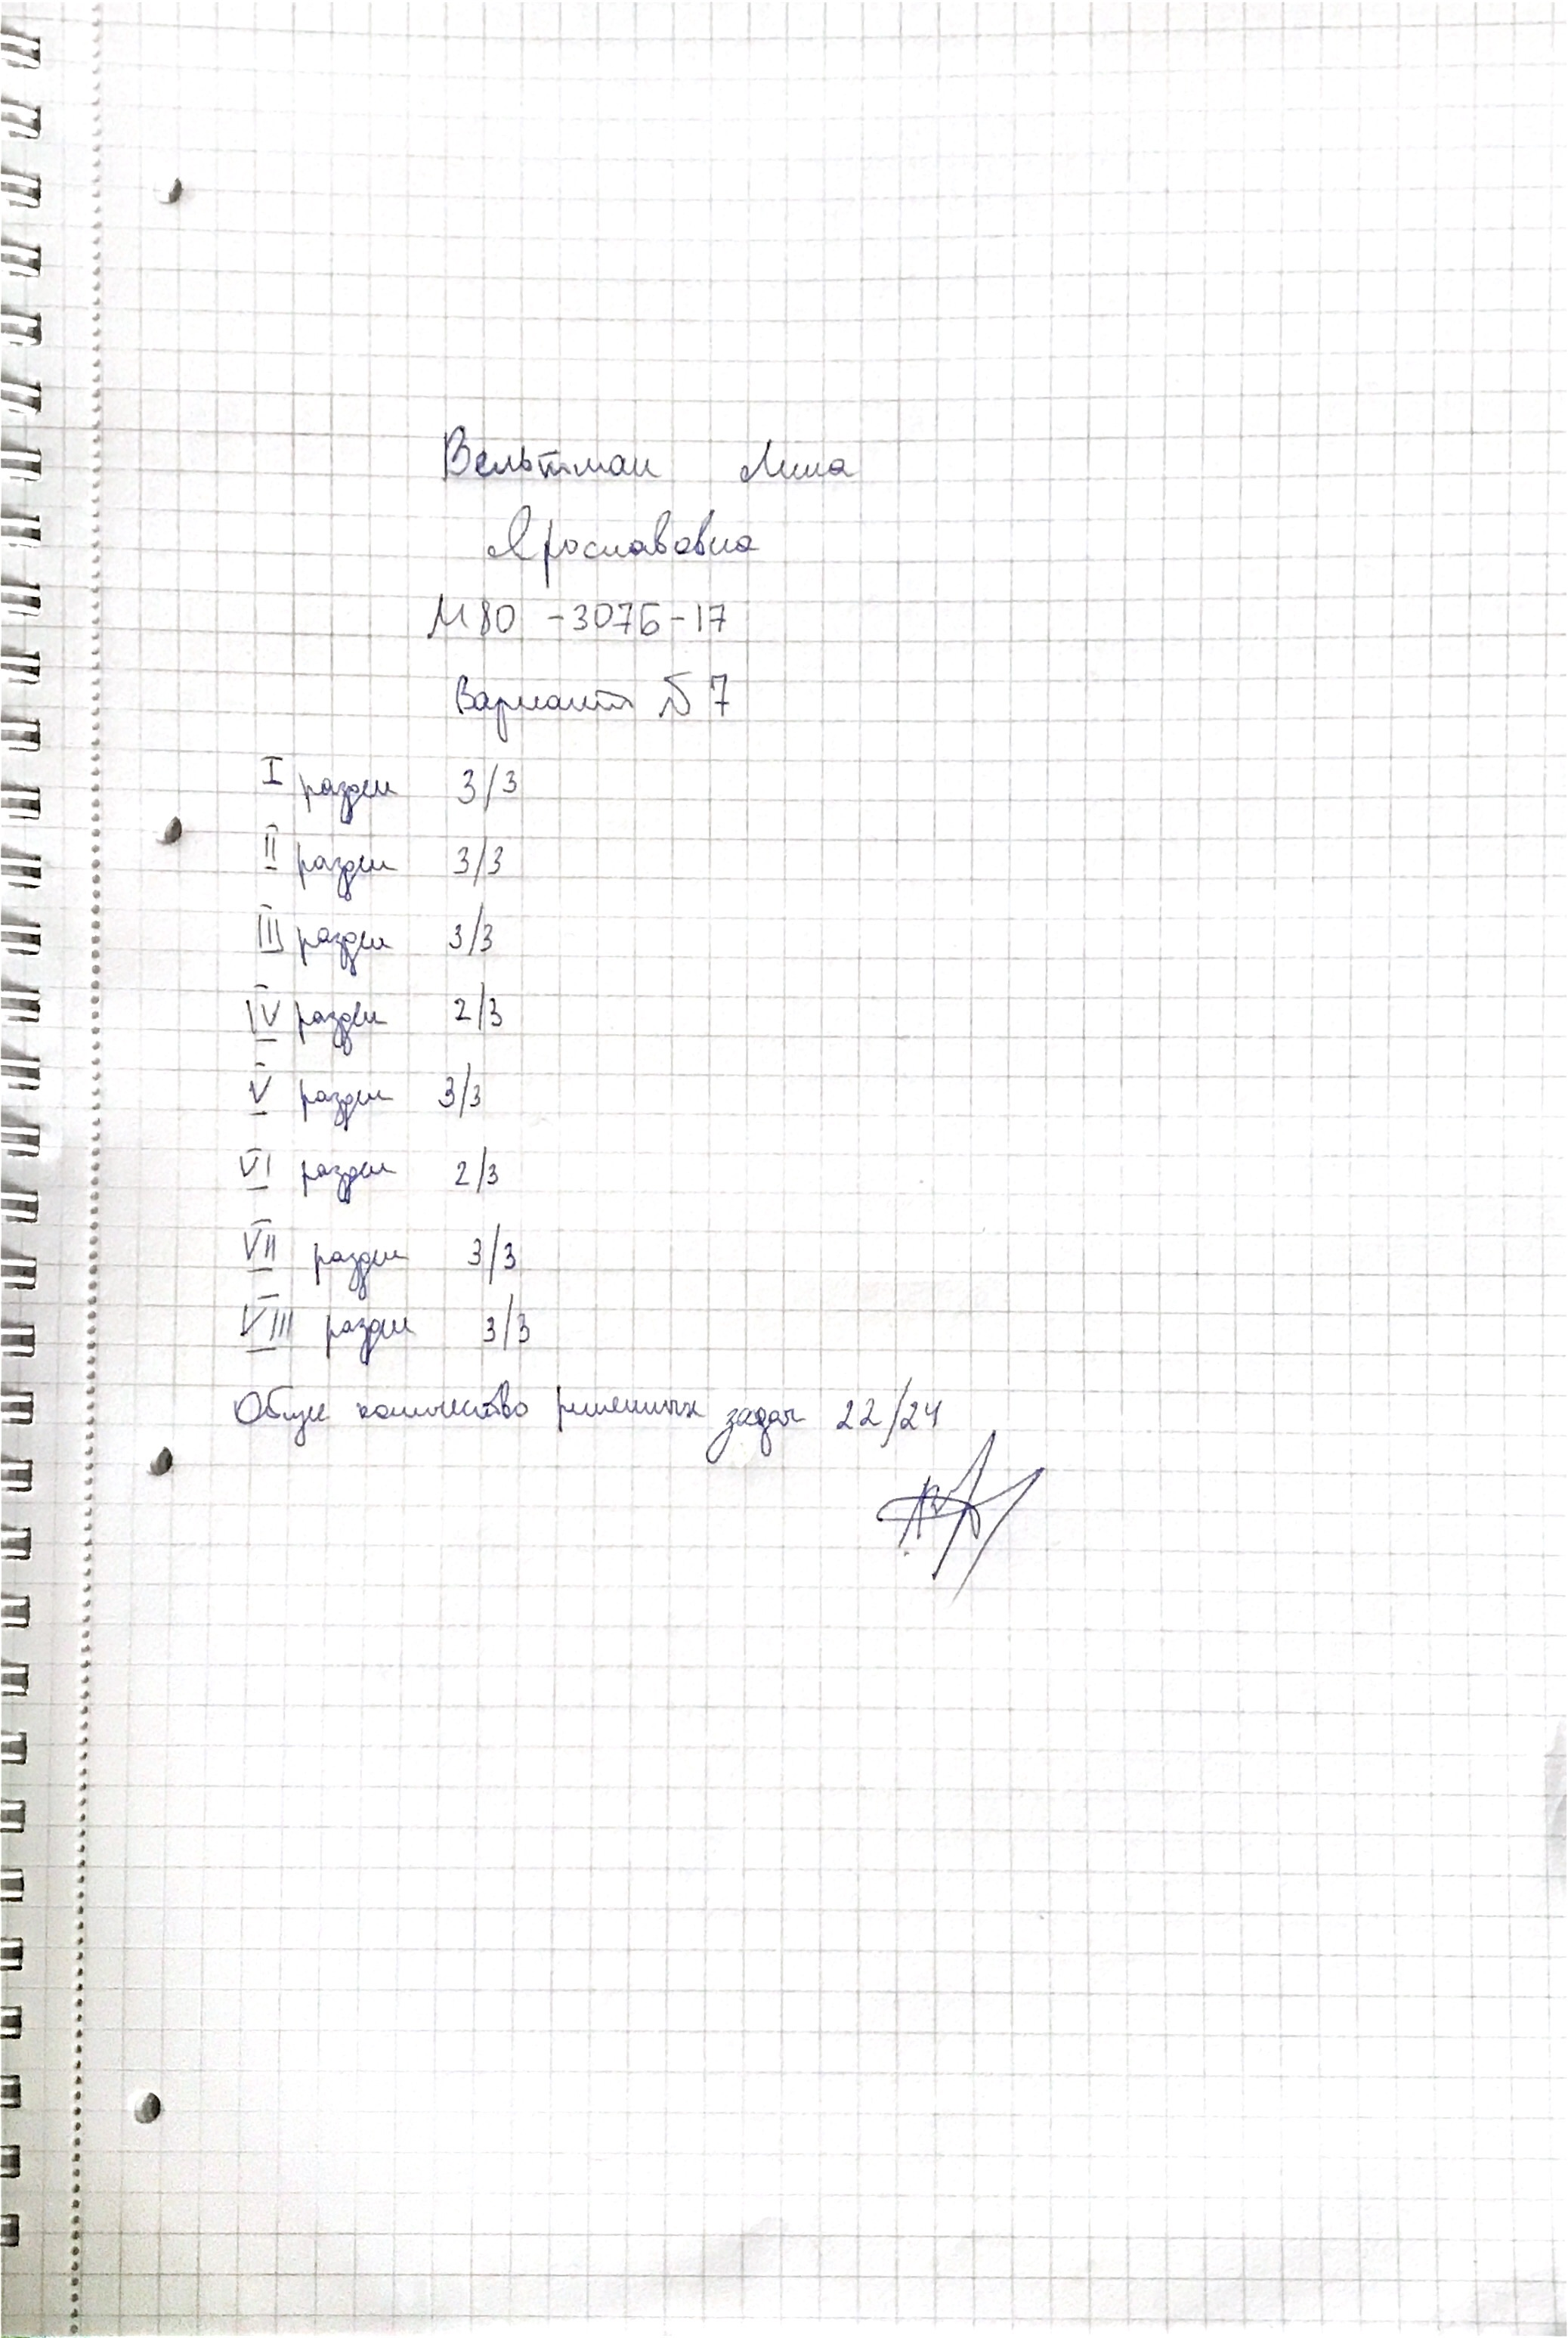
\includegraphics[scale=0.28]{title.jpeg}\\
\vfill
\end{center}
\section{1 раздел}
\begin{center}
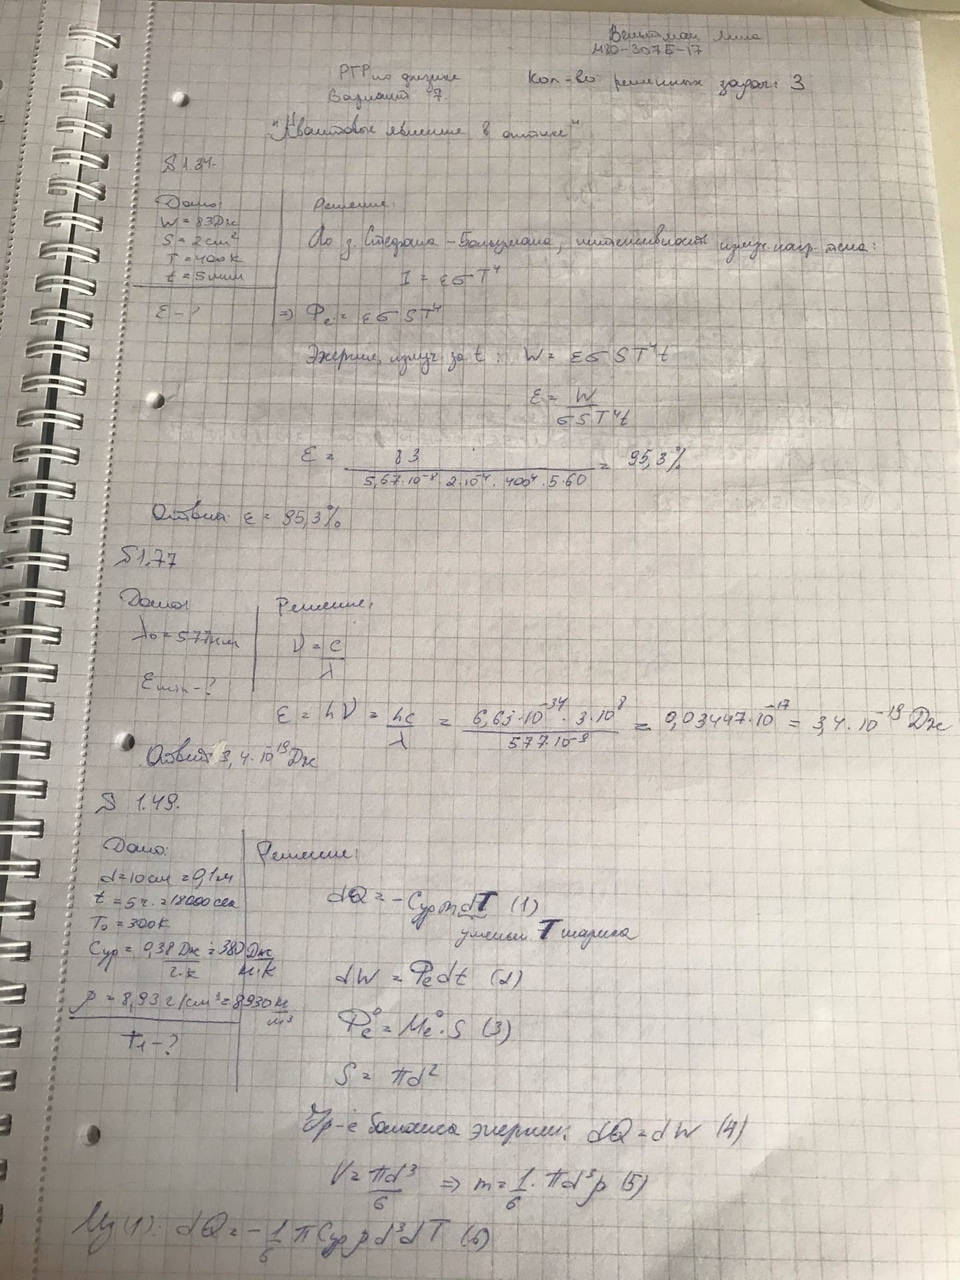
\includegraphics[scale=0.5]{1_1.jpeg}\\
\vfill
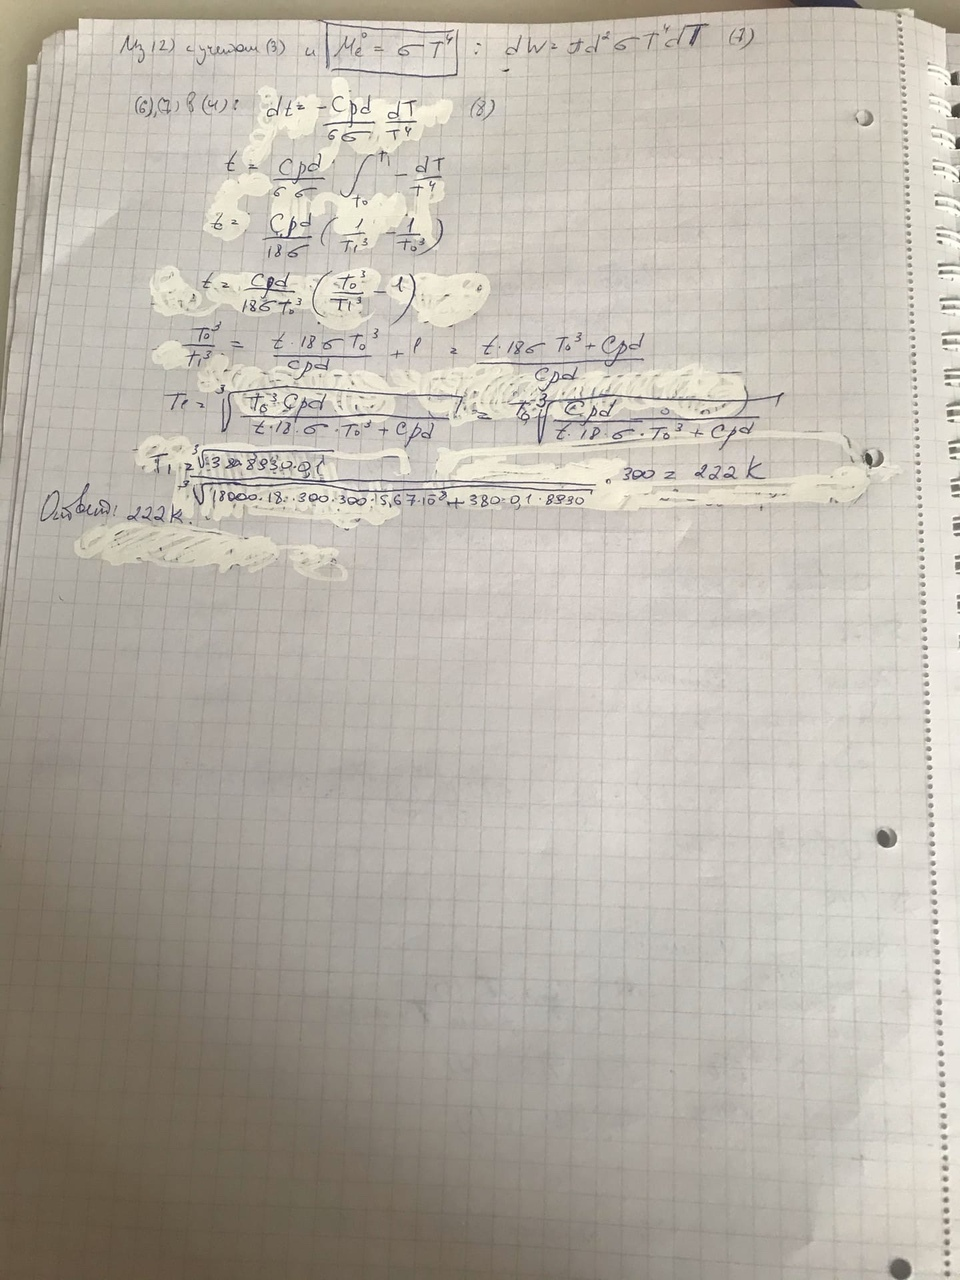
\includegraphics[scale=0.5]{1_2.jpeg}\\
\end{center}
\section{2 раздел}
\begin{center}
\includegraphics[scale=0.18]{2_2.jpeg}\\
\vfill
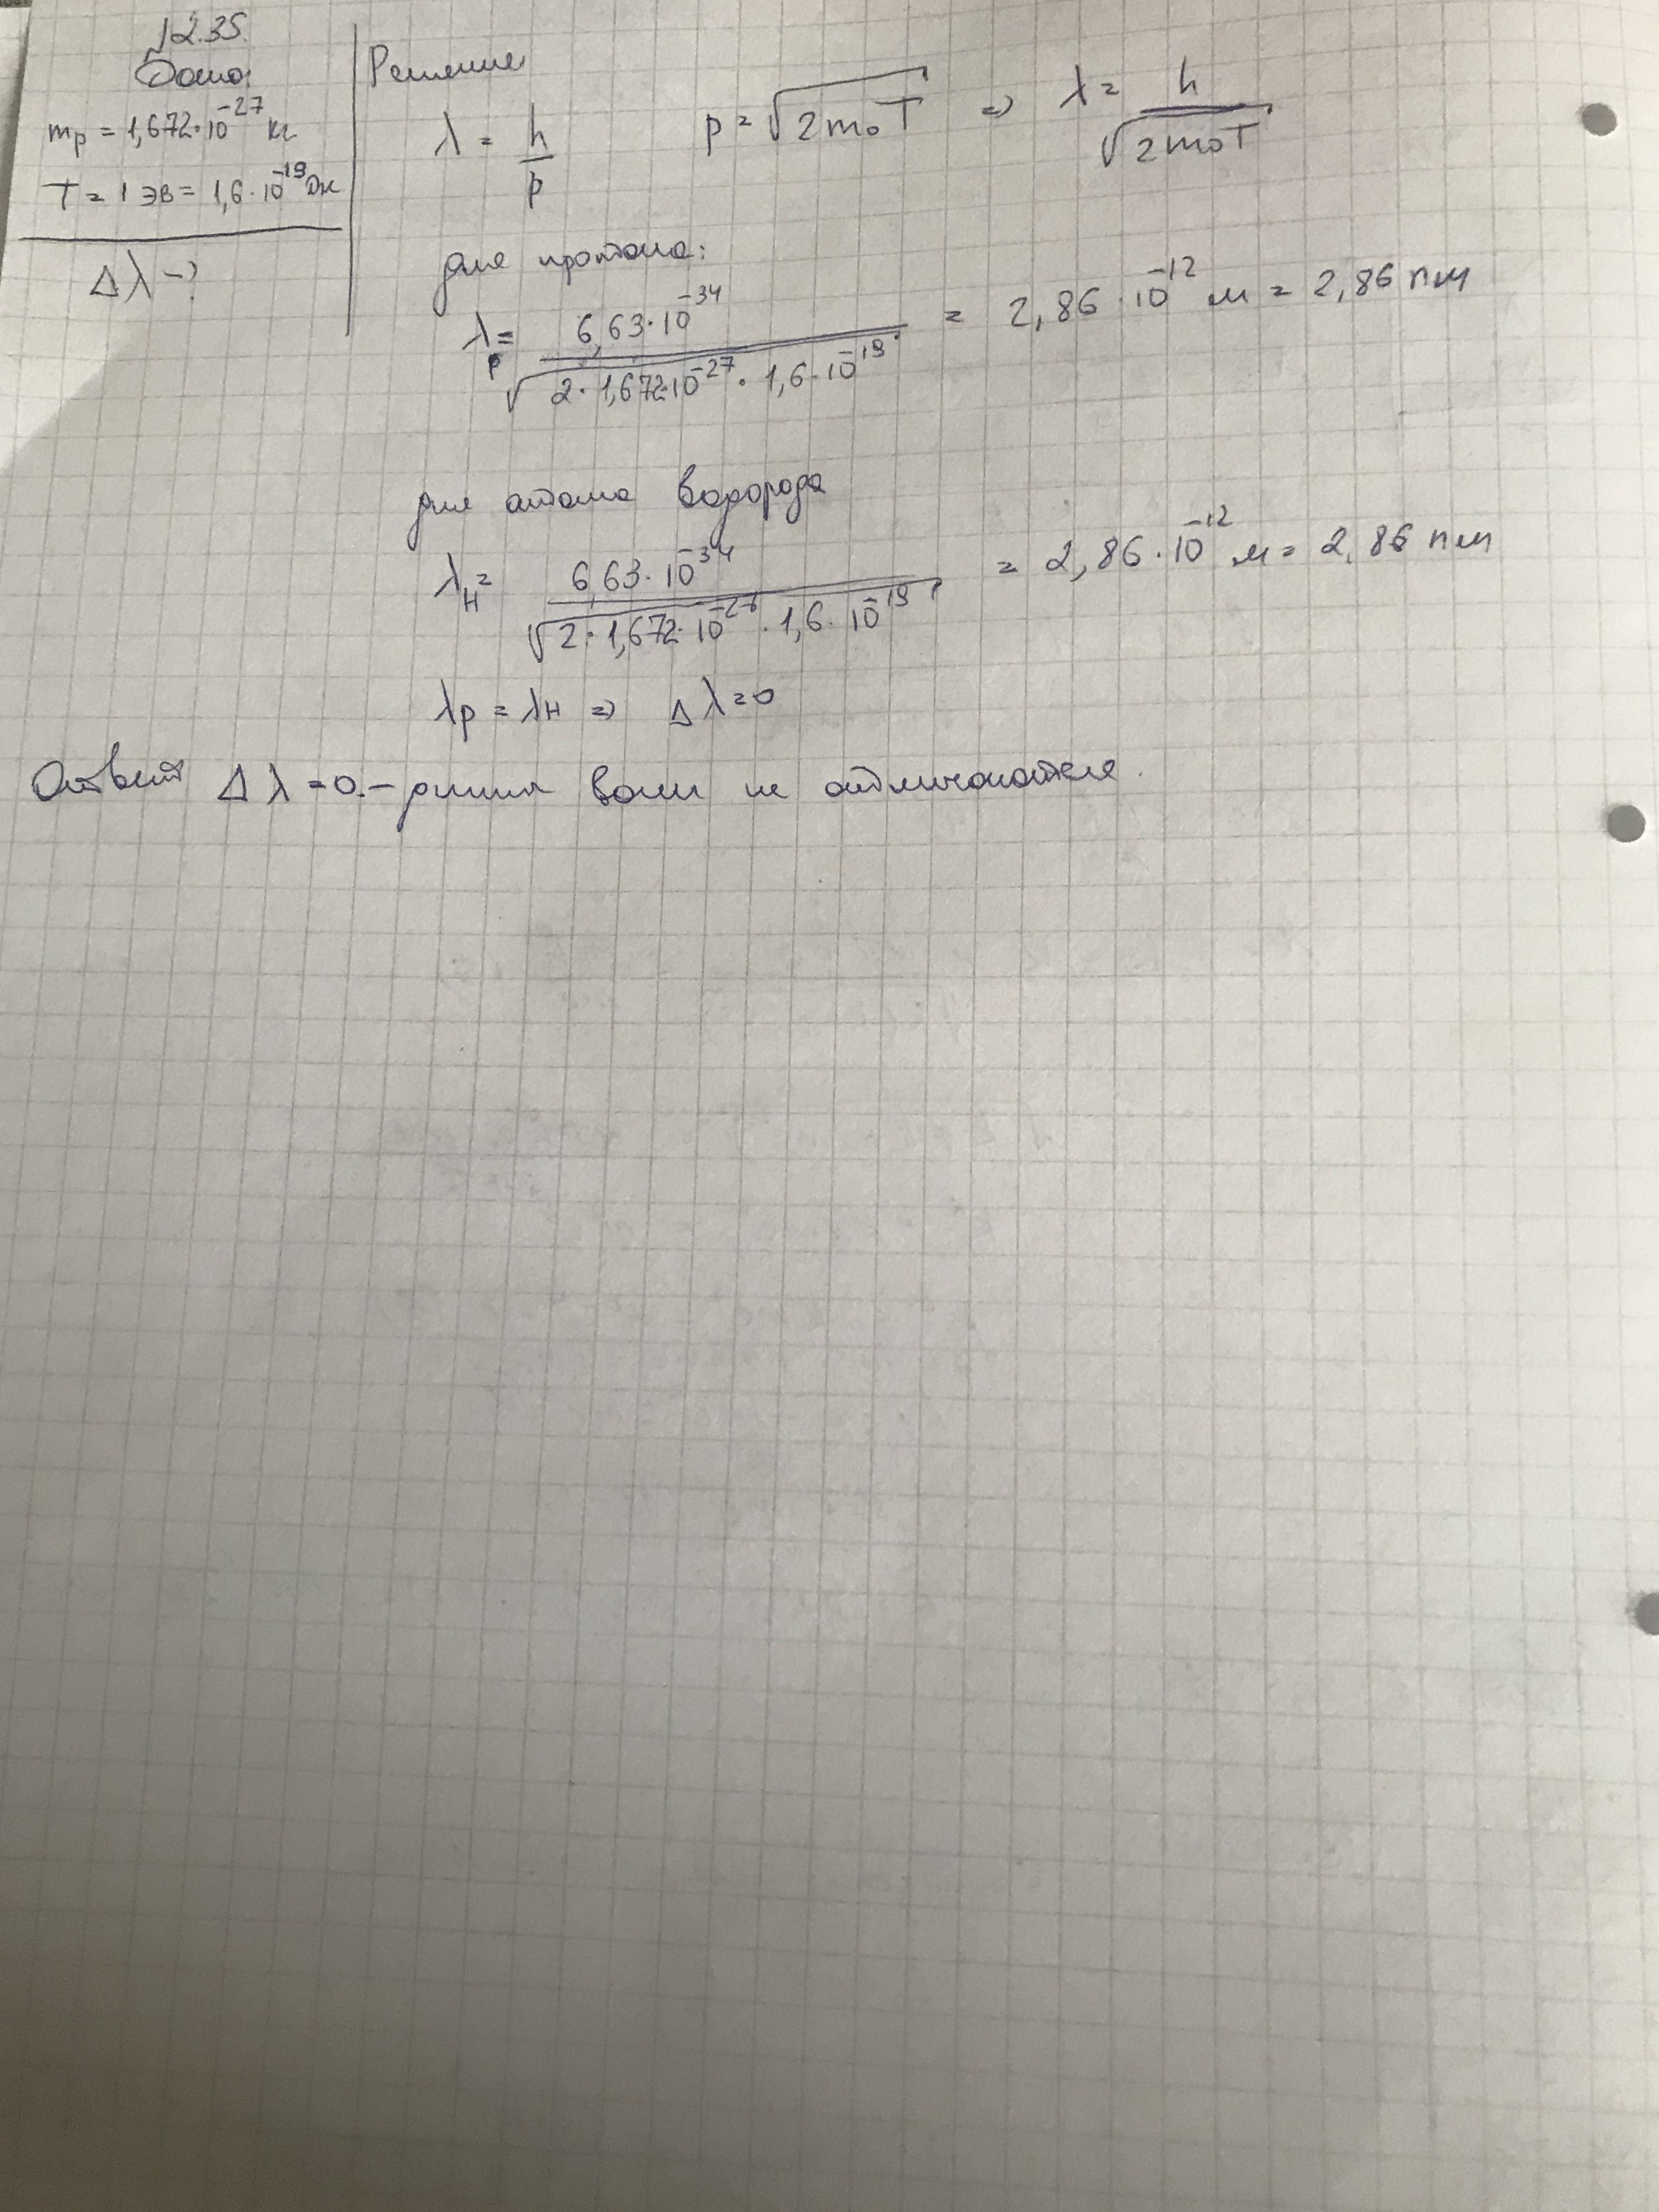
\includegraphics[scale=0.18]{2_1.jpeg}\\
\end{center}
\section{3 раздел}
\begin{center}
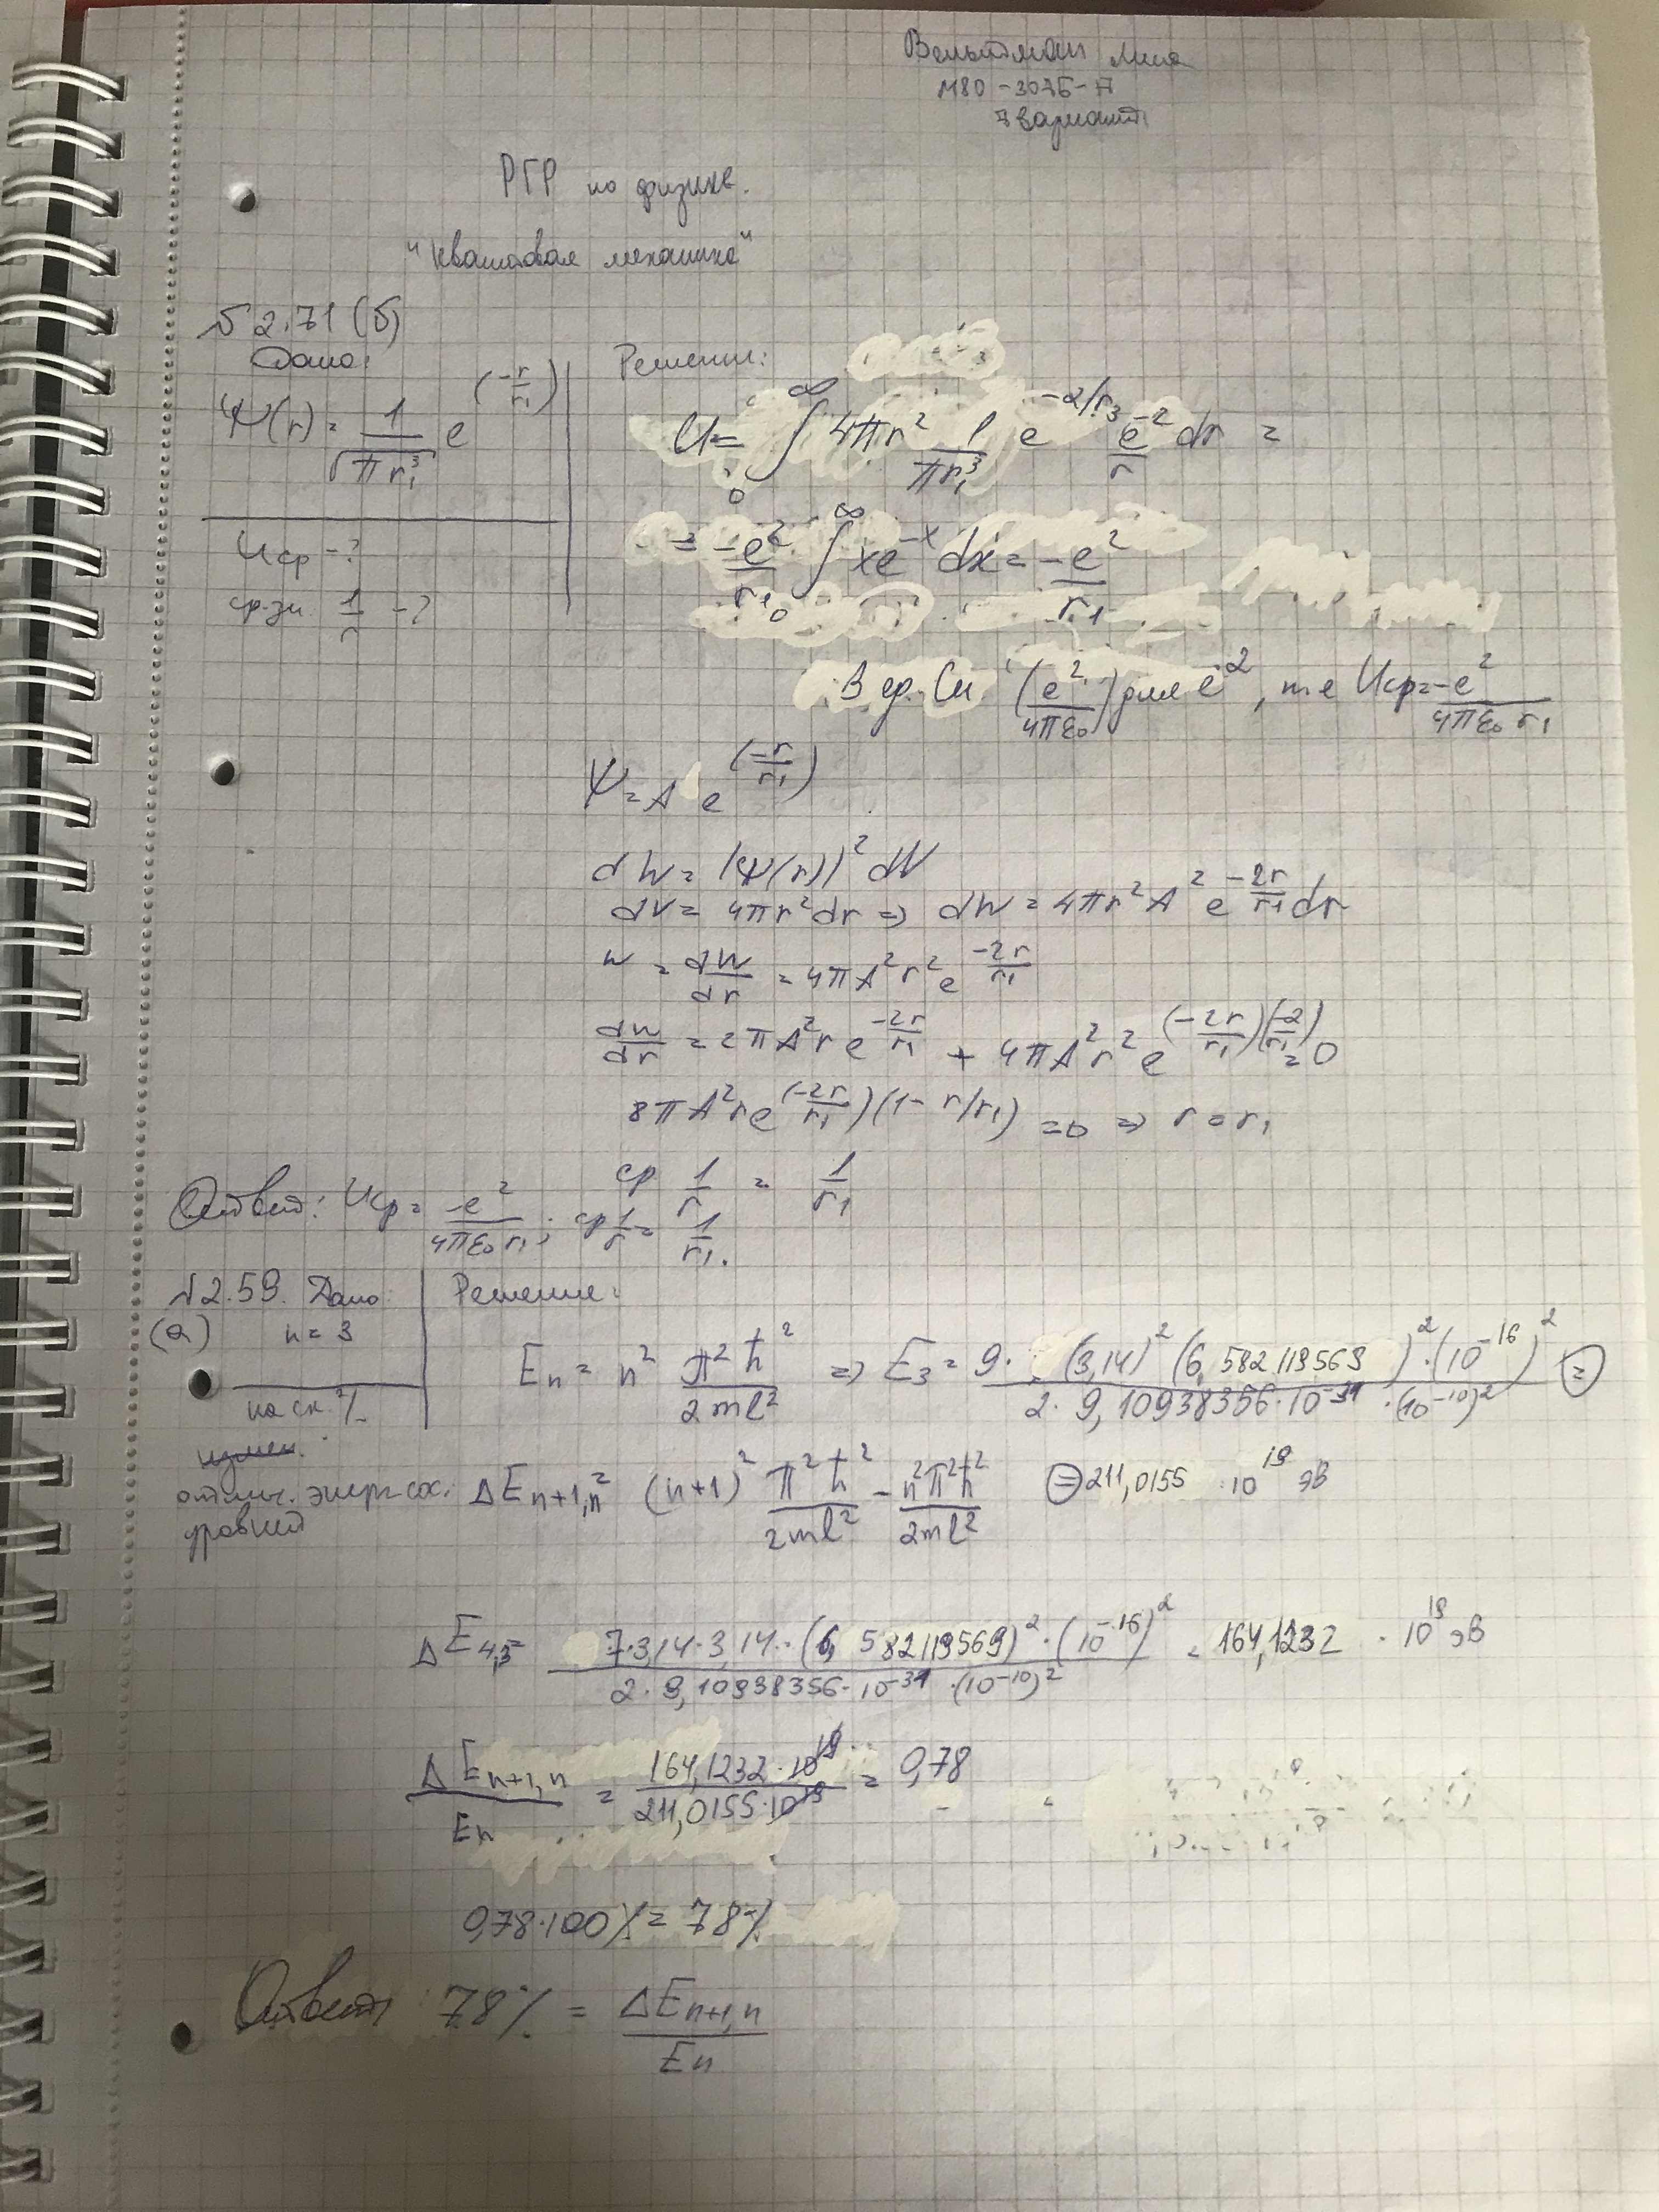
\includegraphics[scale=0.18]{3_1.jpeg}\\
\vfill
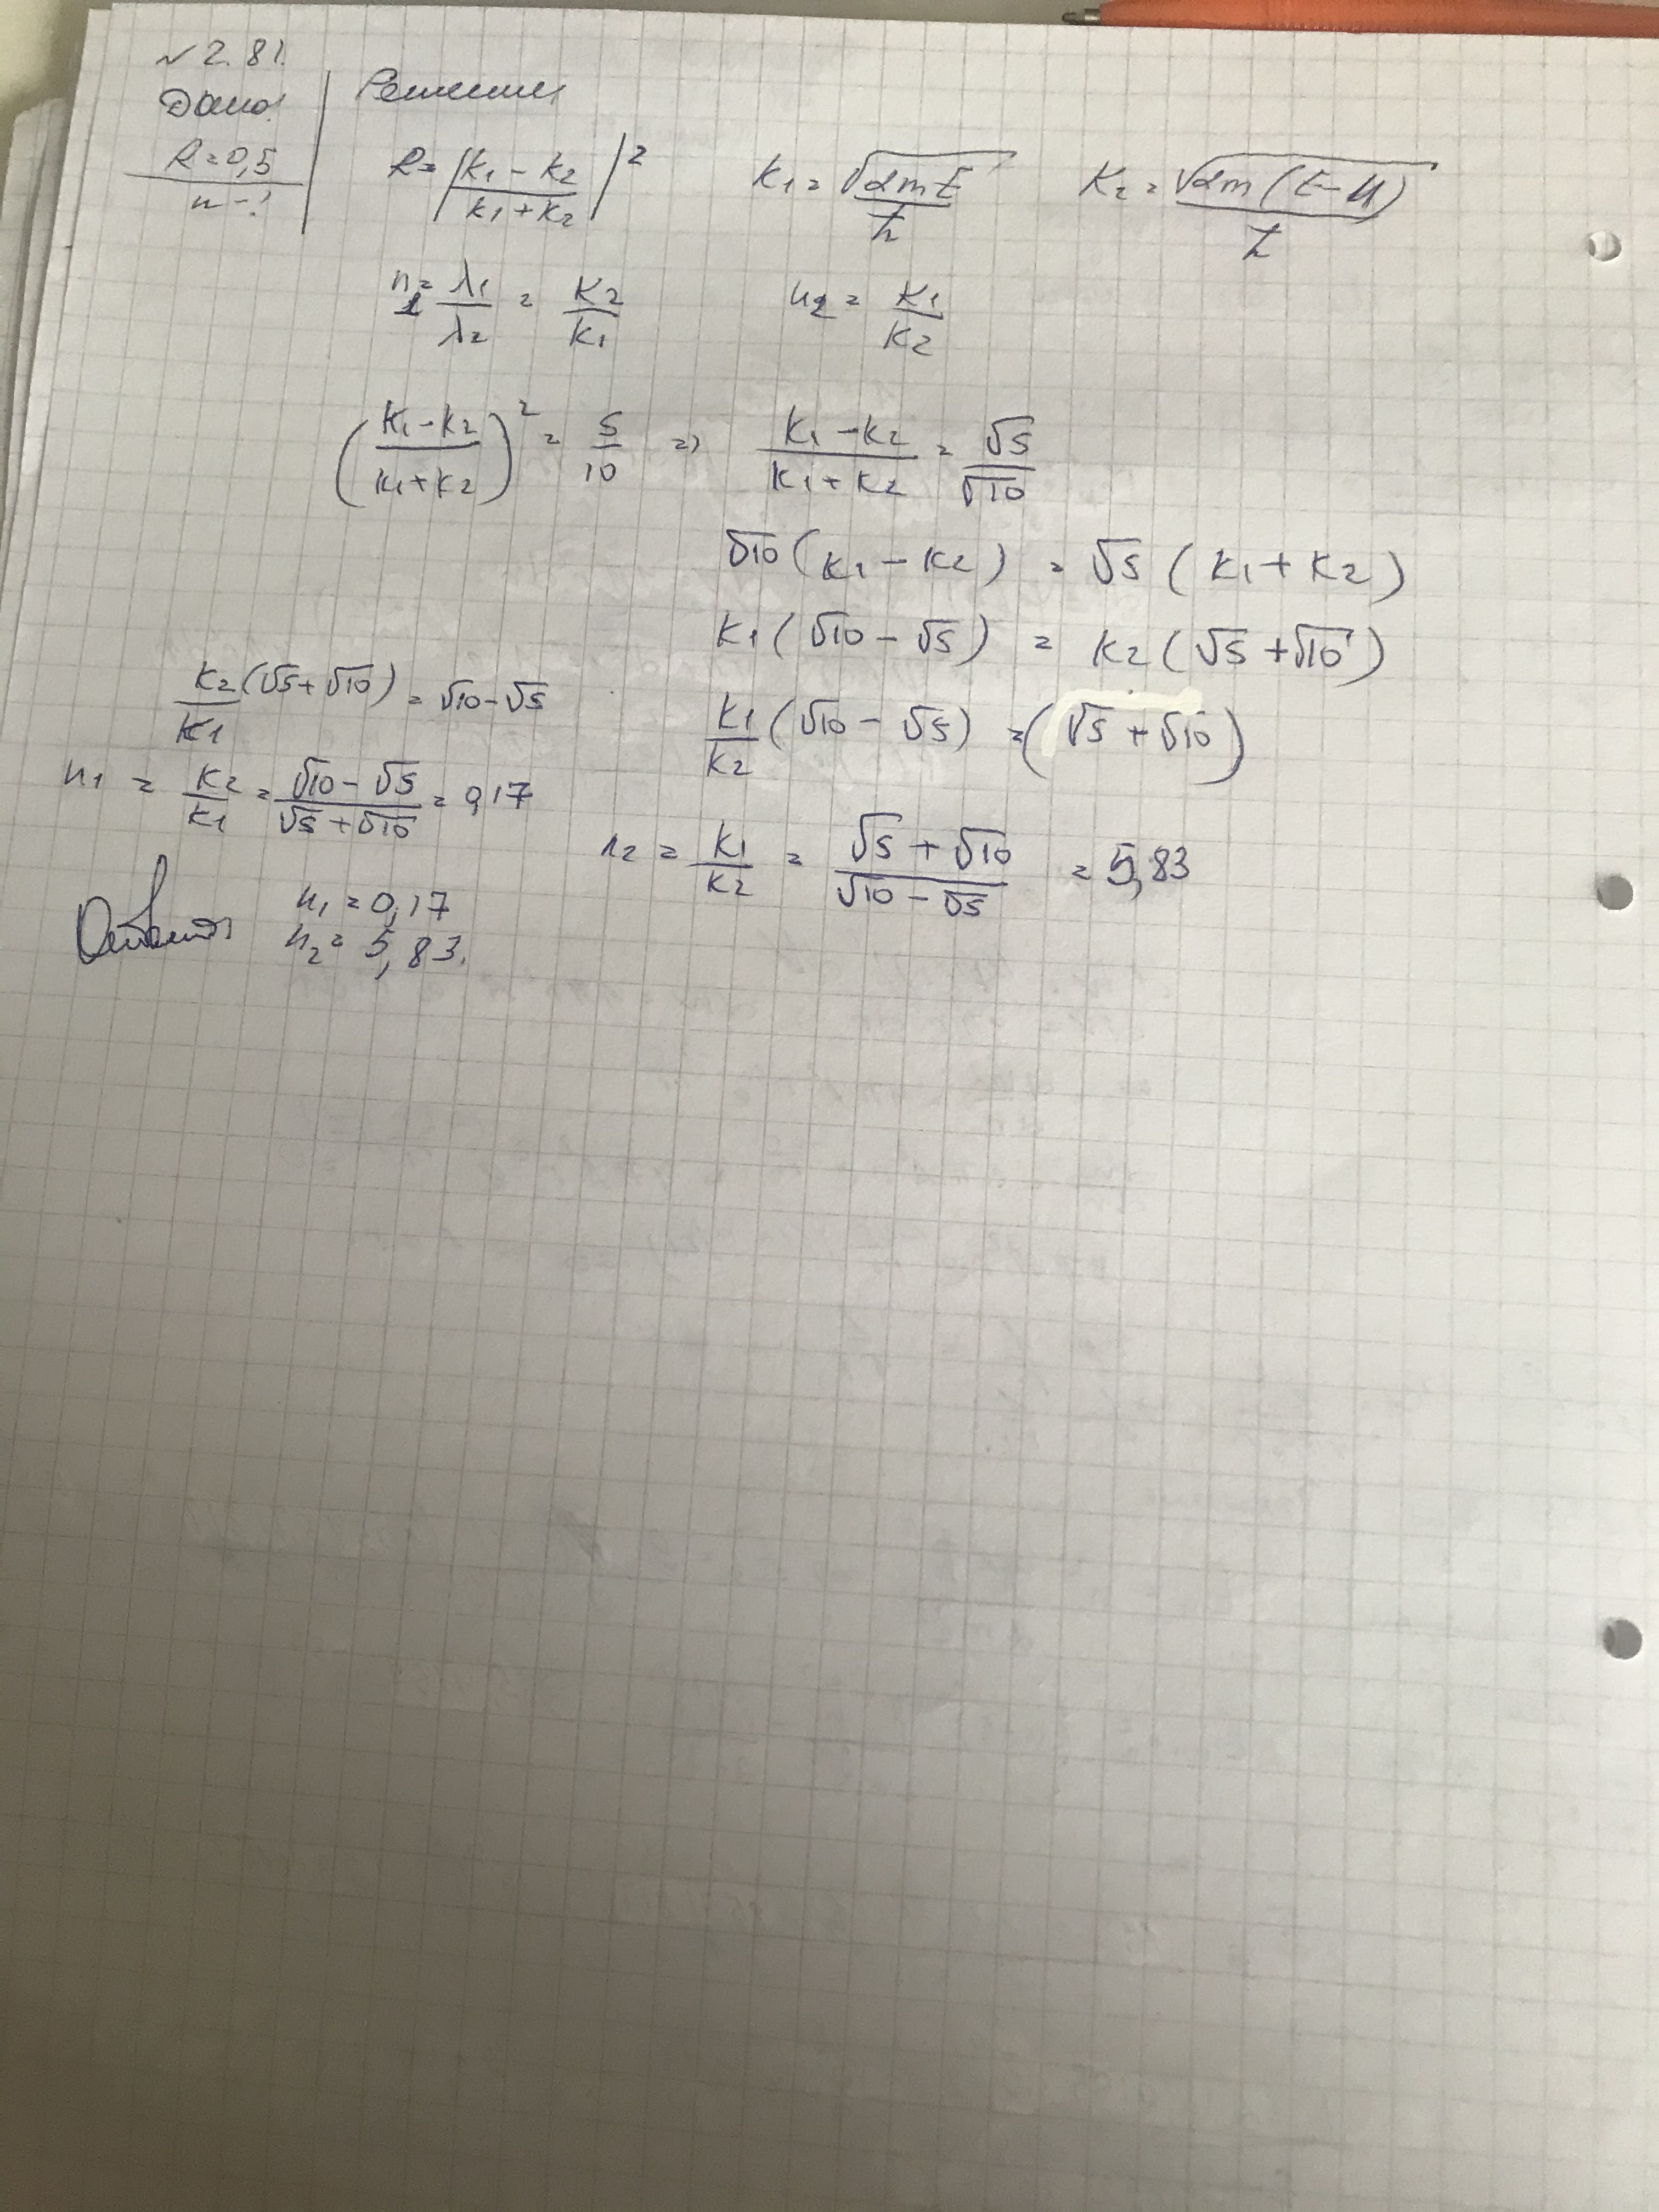
\includegraphics[scale=0.18]{3_2.jpeg}\\
\end{center}
\section{4 раздел}
\begin{center}
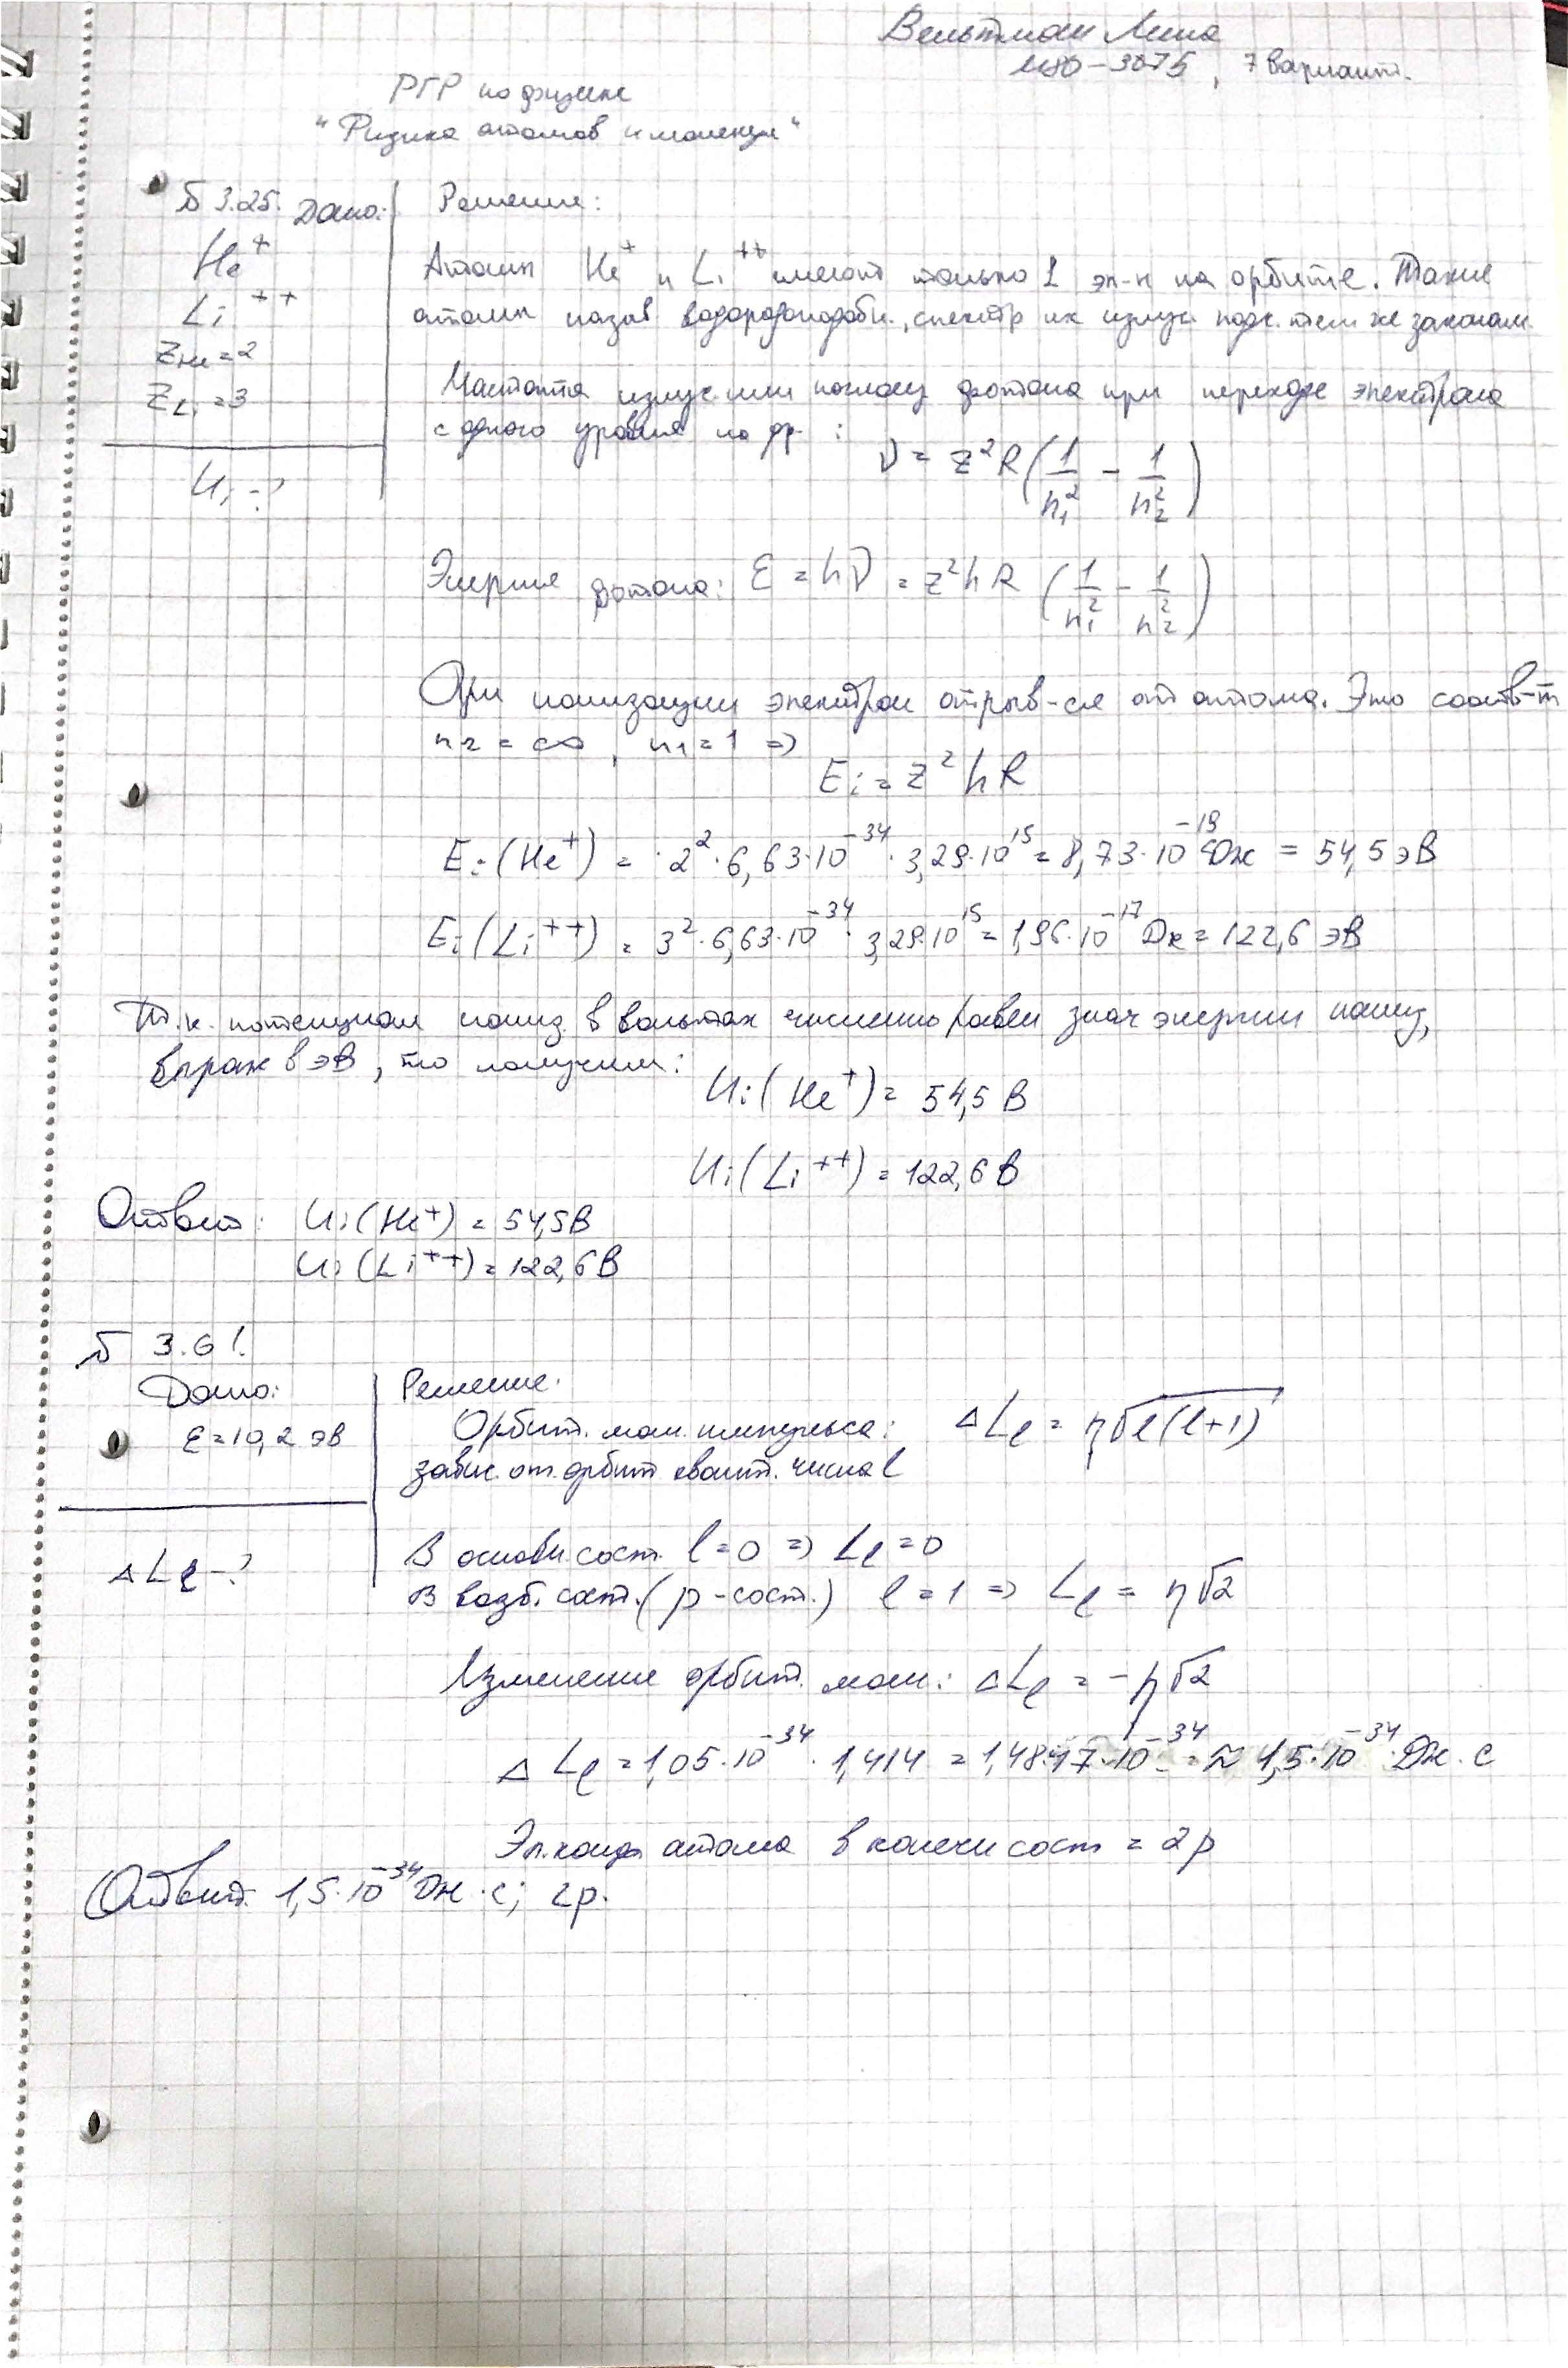
\includegraphics[scale=0.2]{4_1.jpeg}\\
\vfill
\end{center}
\section{5 раздел}
\begin{center}
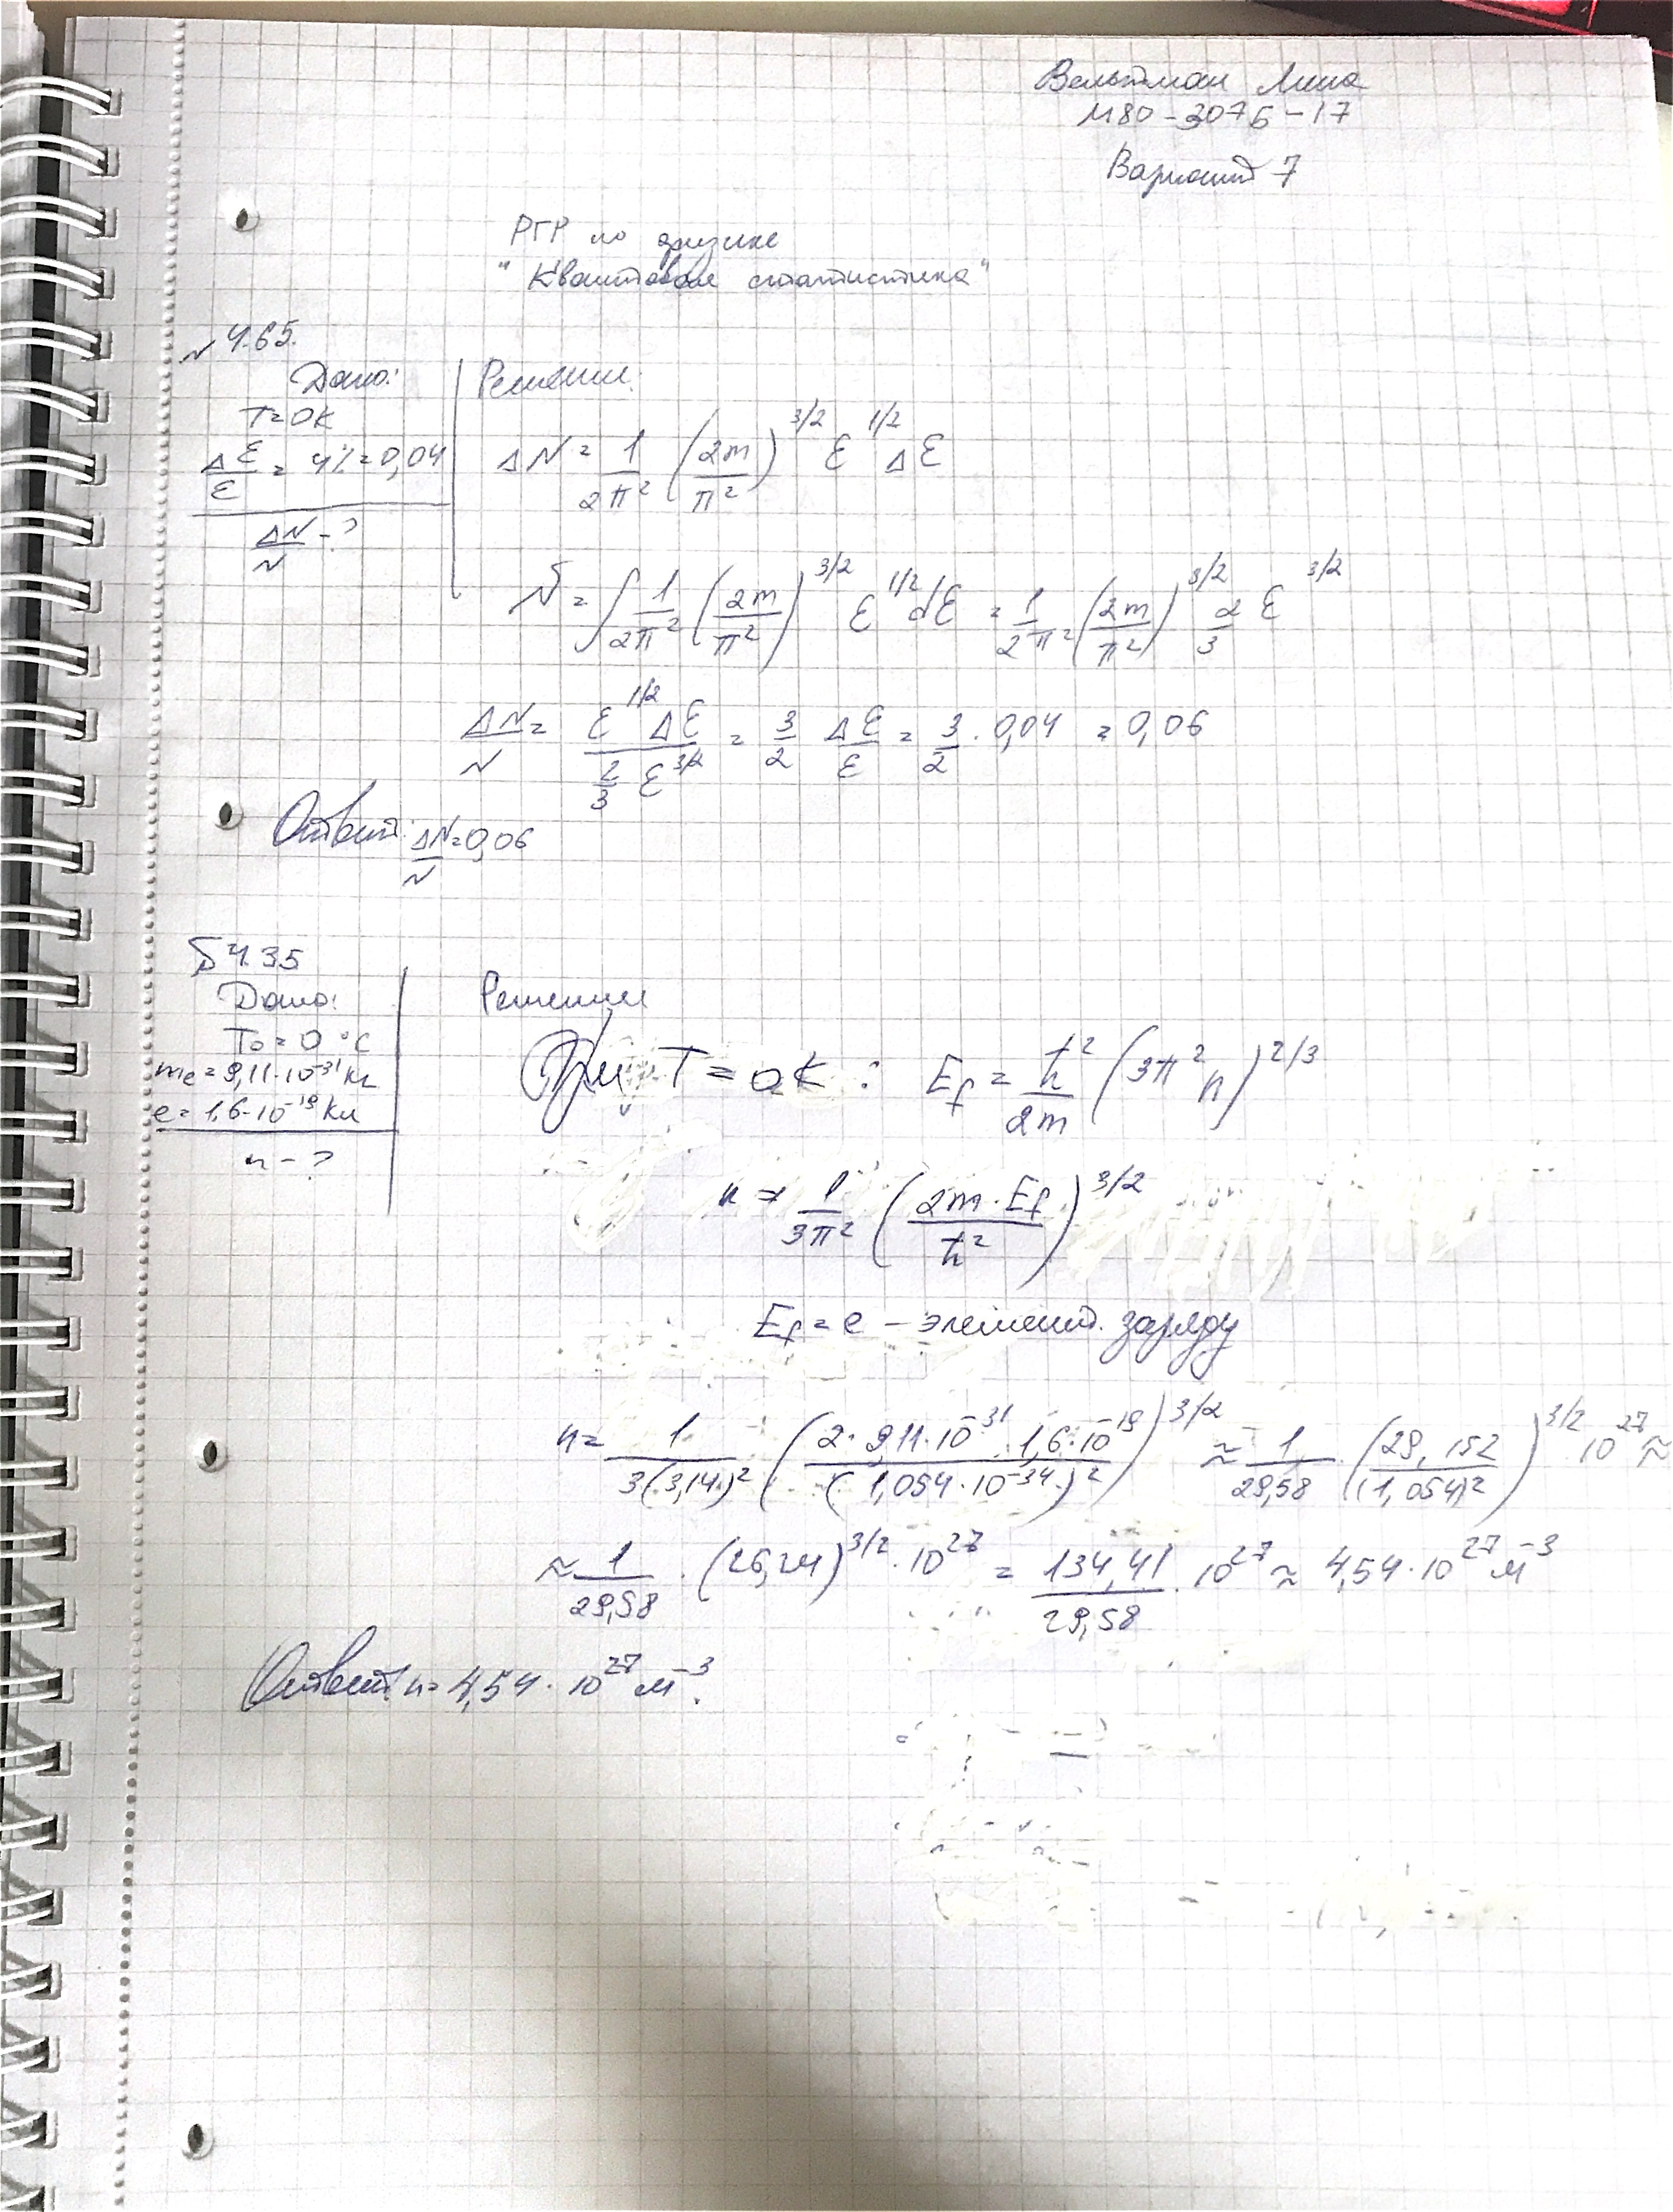
\includegraphics[scale=0.18]{5_1.jpeg}\\
\vfill
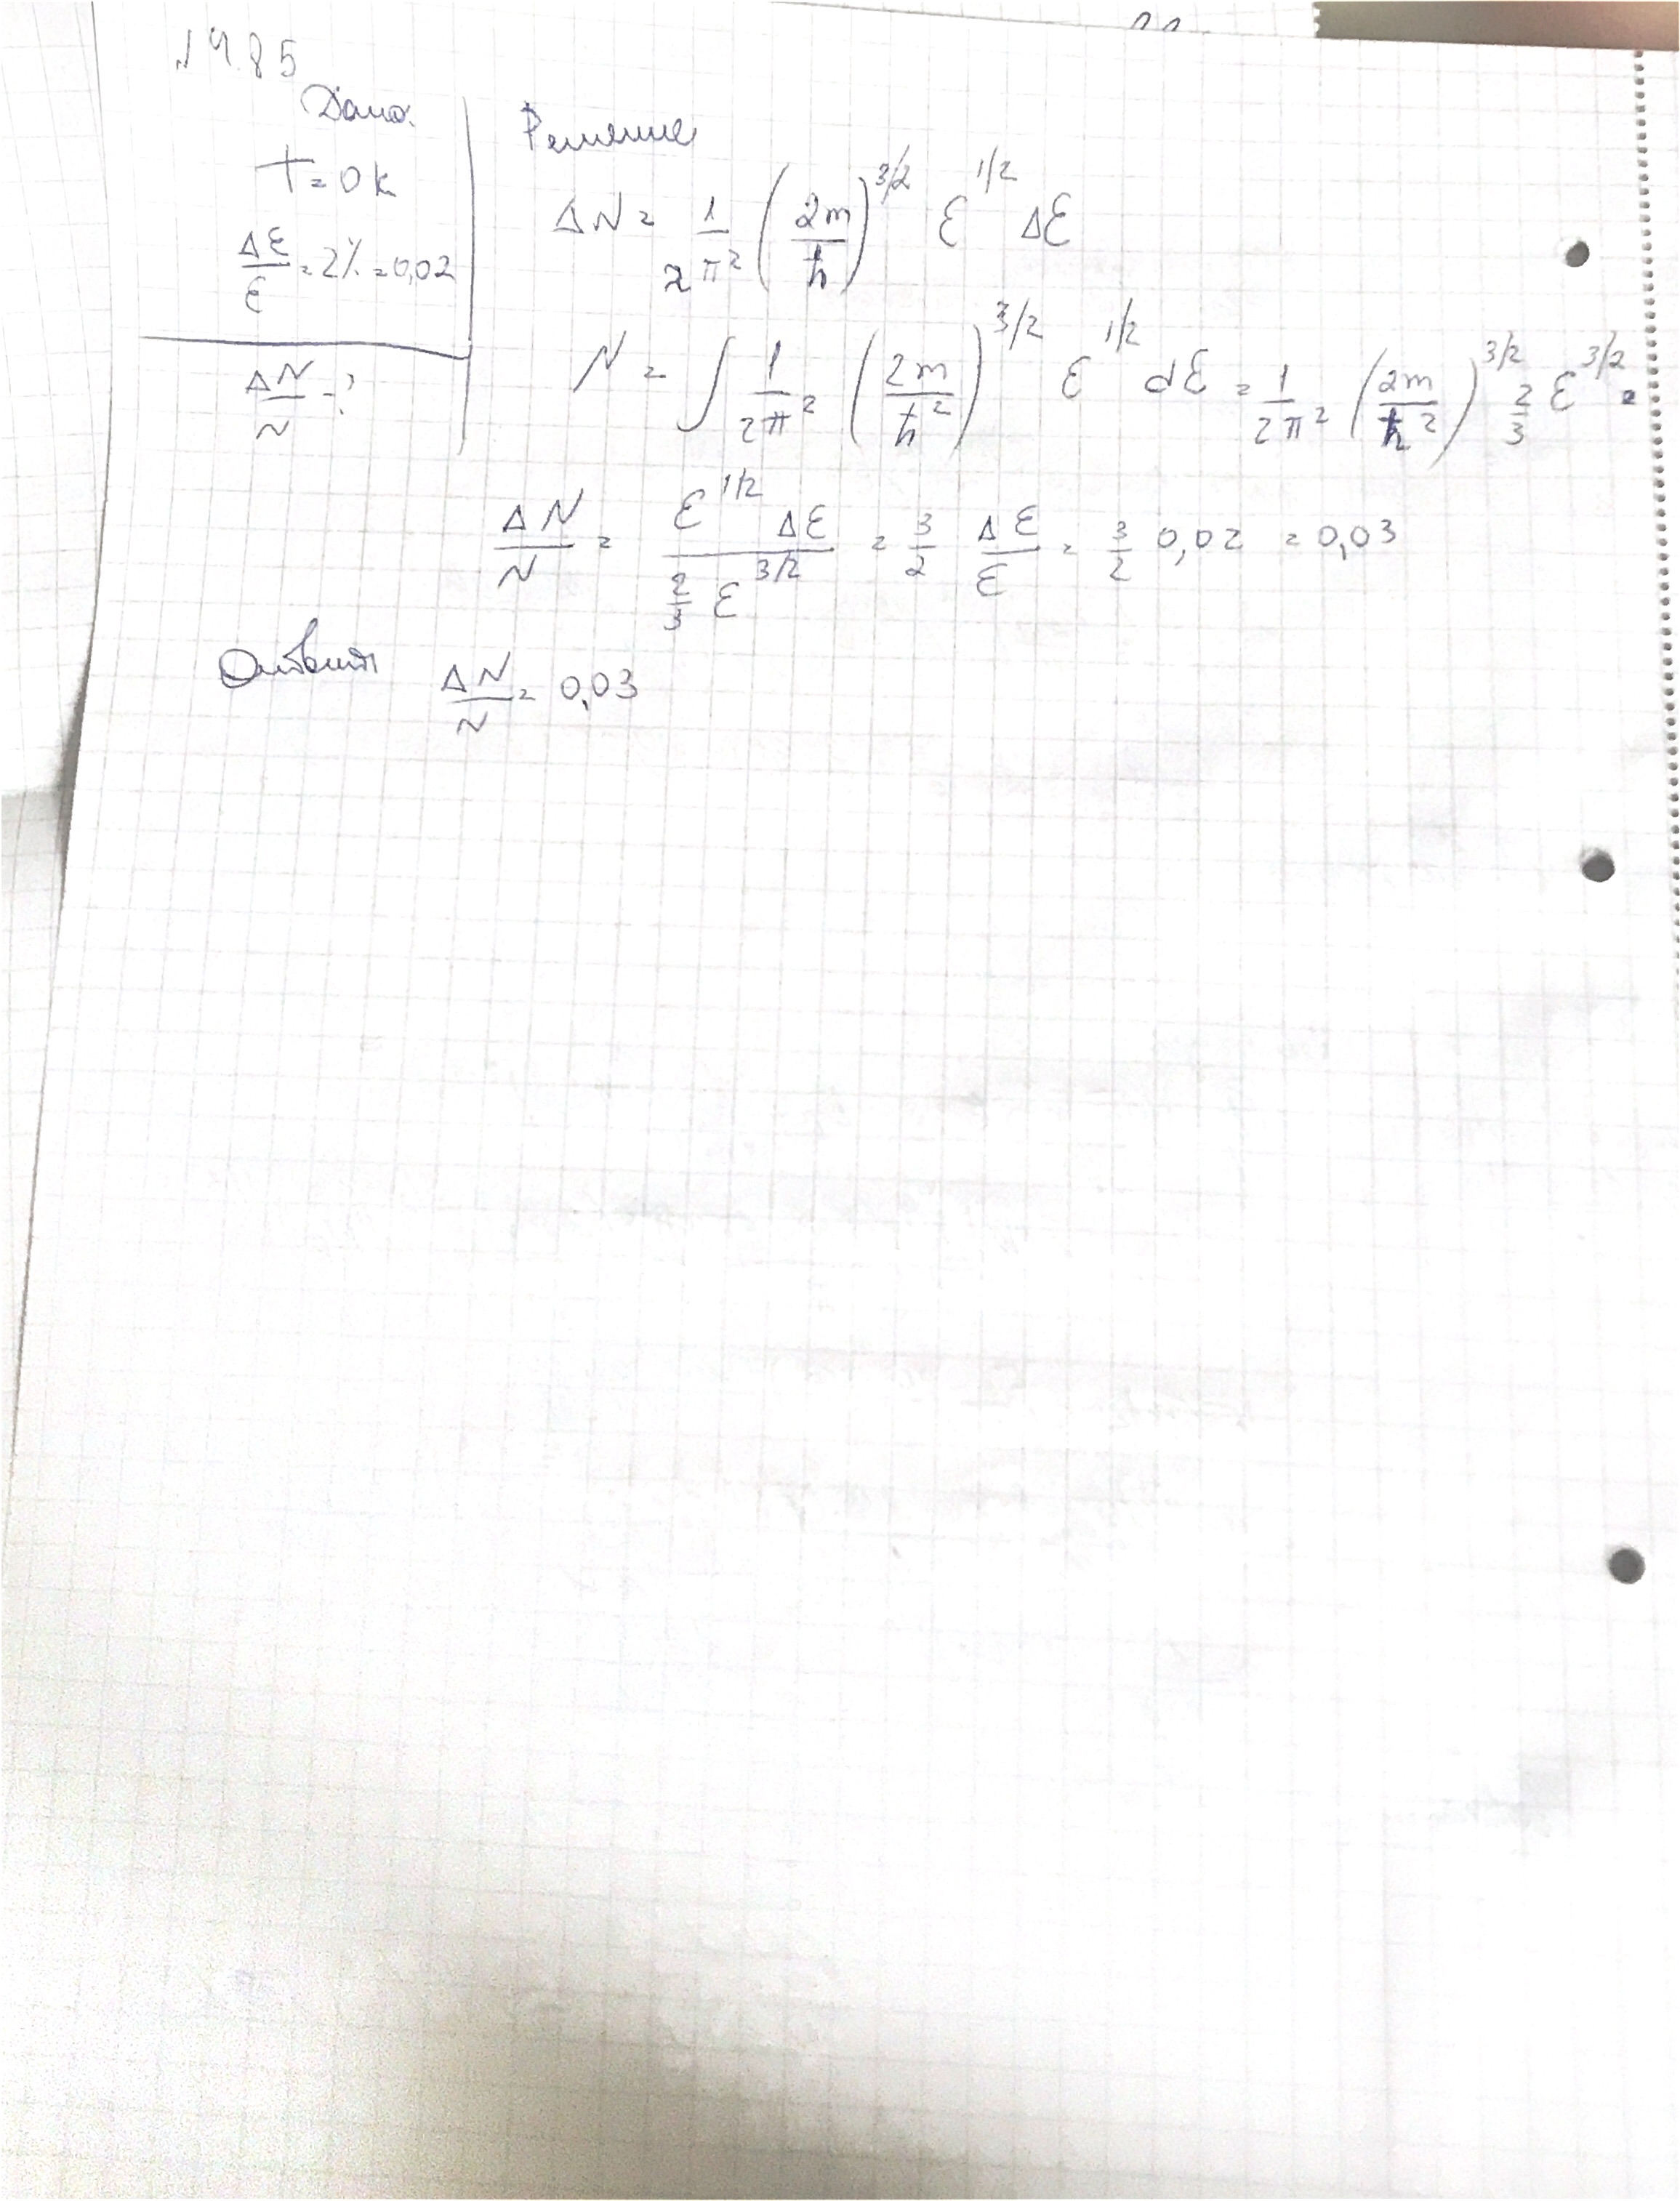
\includegraphics[scale=0.2]{5_2.jpeg}\\
\end{center}
\section{6 раздел}
\begin{center}
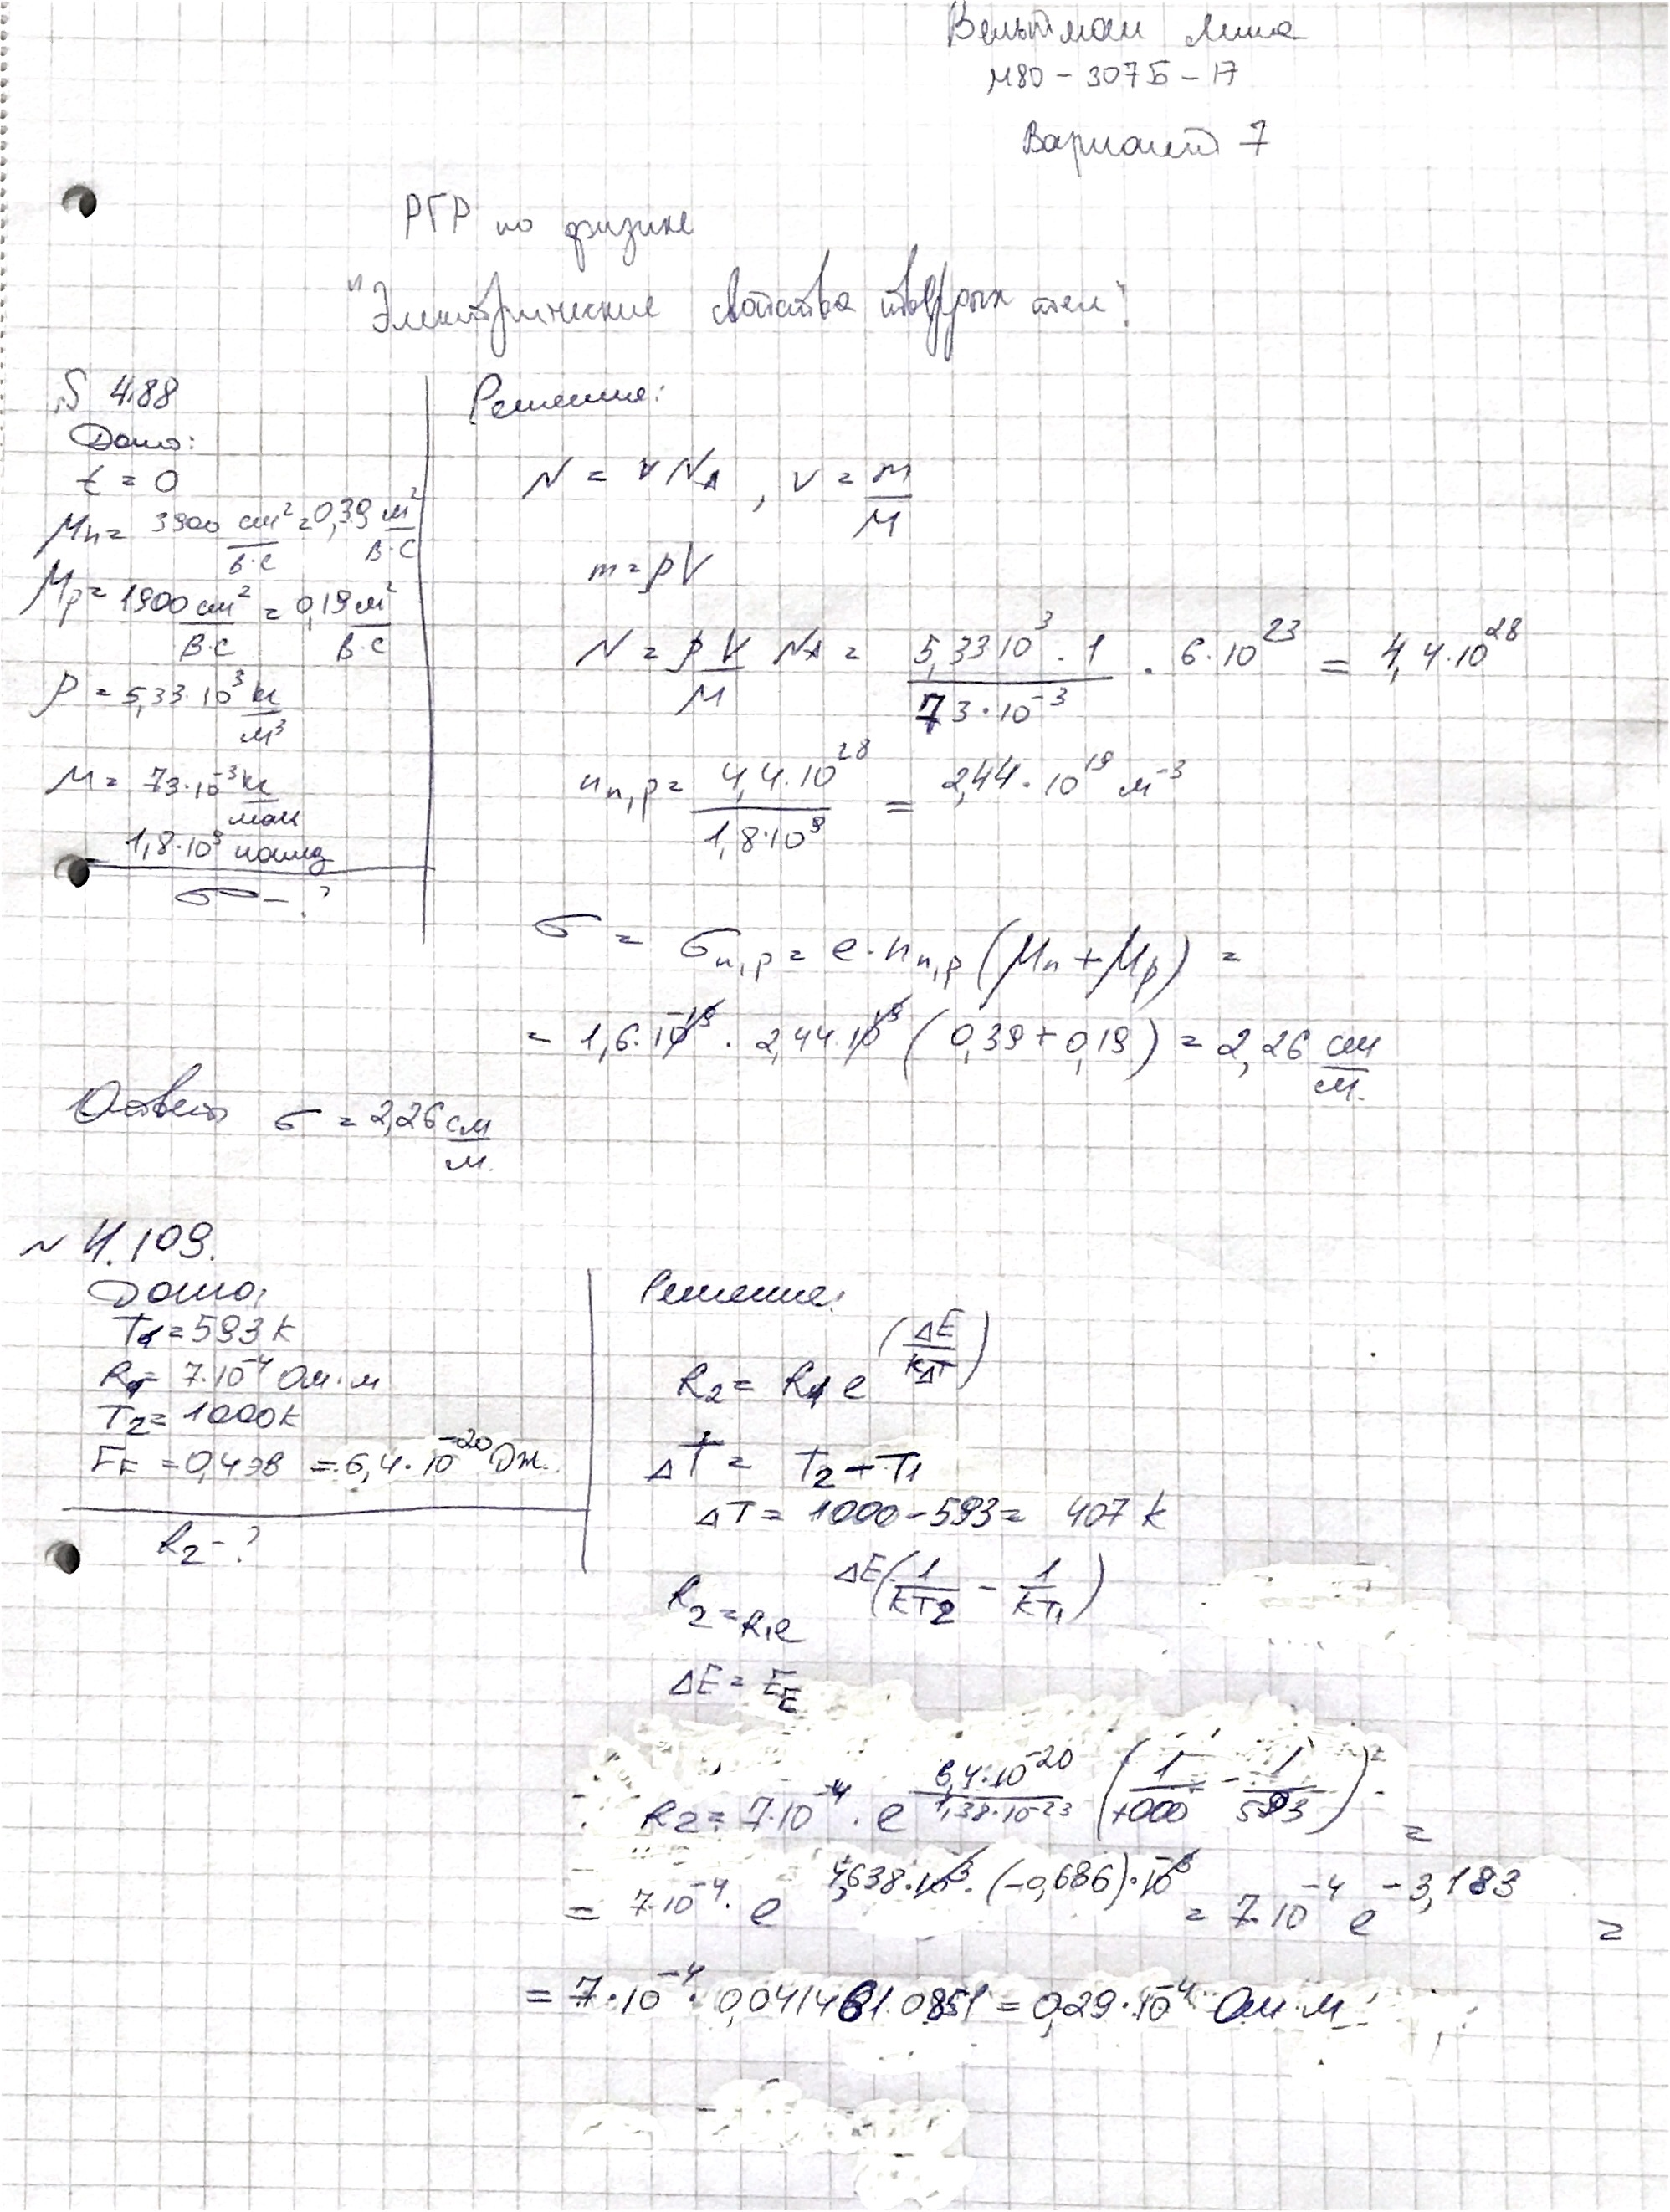
\includegraphics[scale=0.2]{6_1.jpeg}\\
\vfill
\end{center}
\section{7 раздел}
\begin{center}
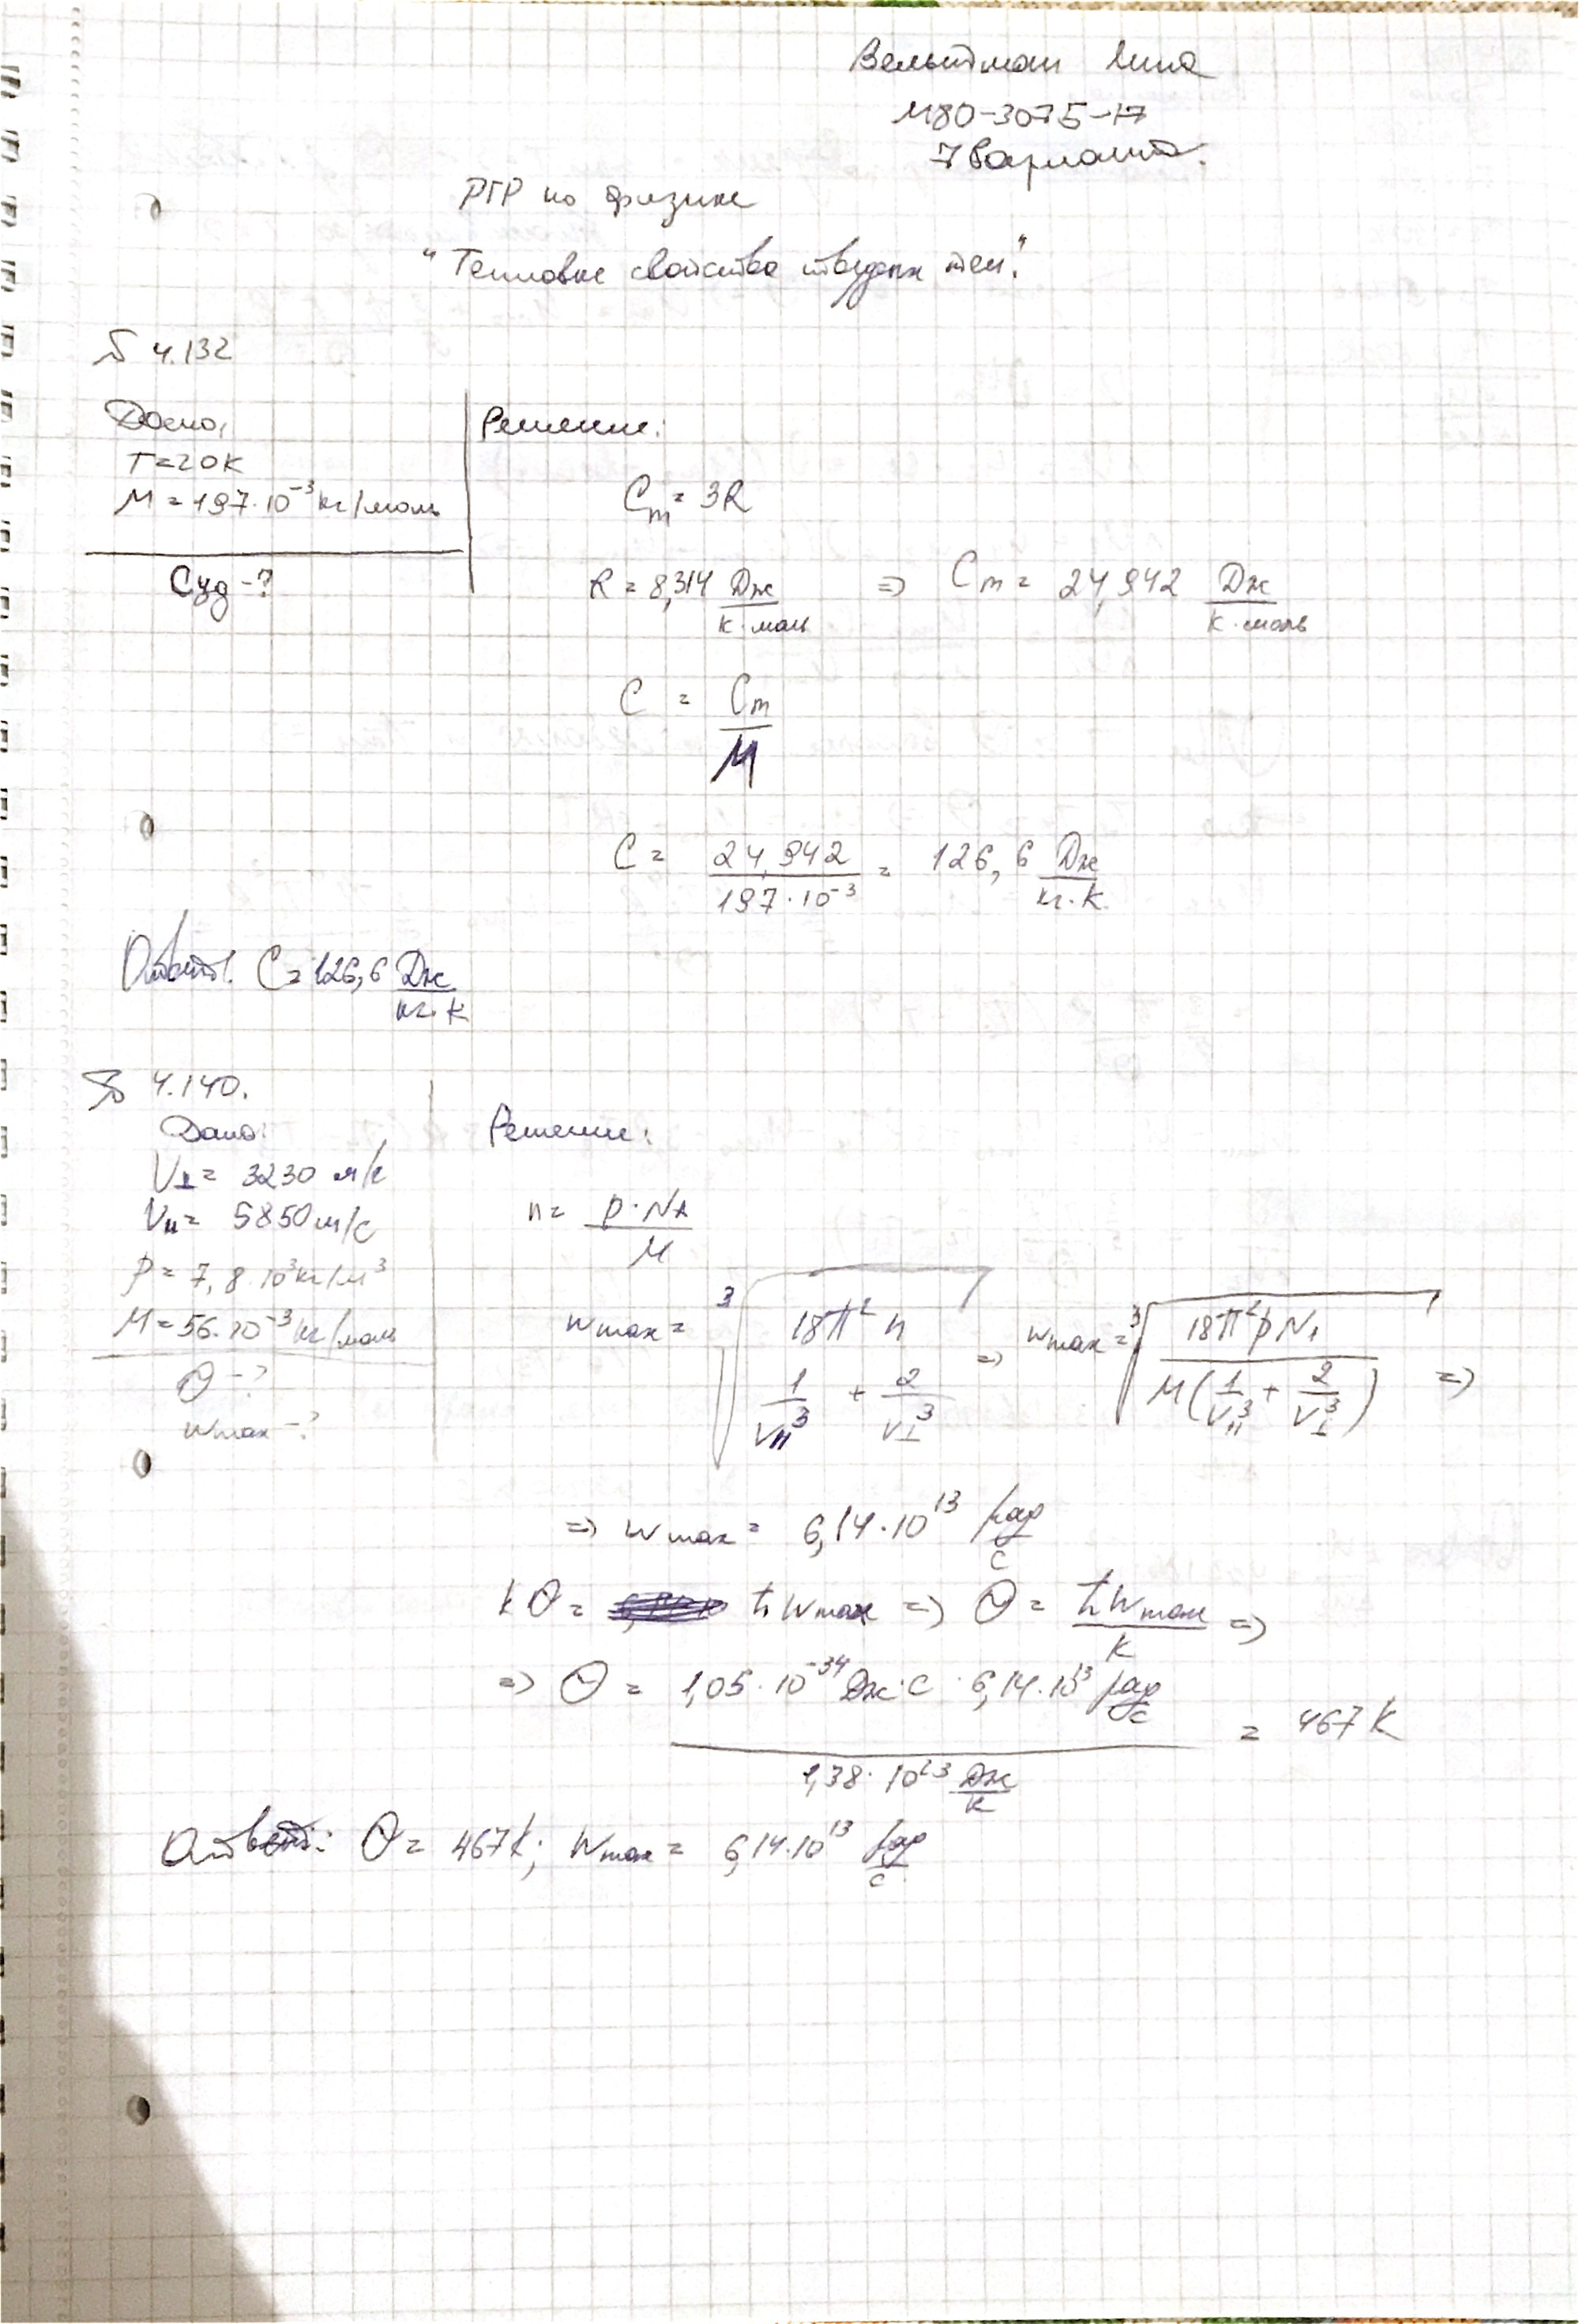
\includegraphics[scale=0.2]{7_1.jpeg}\\
\vfill
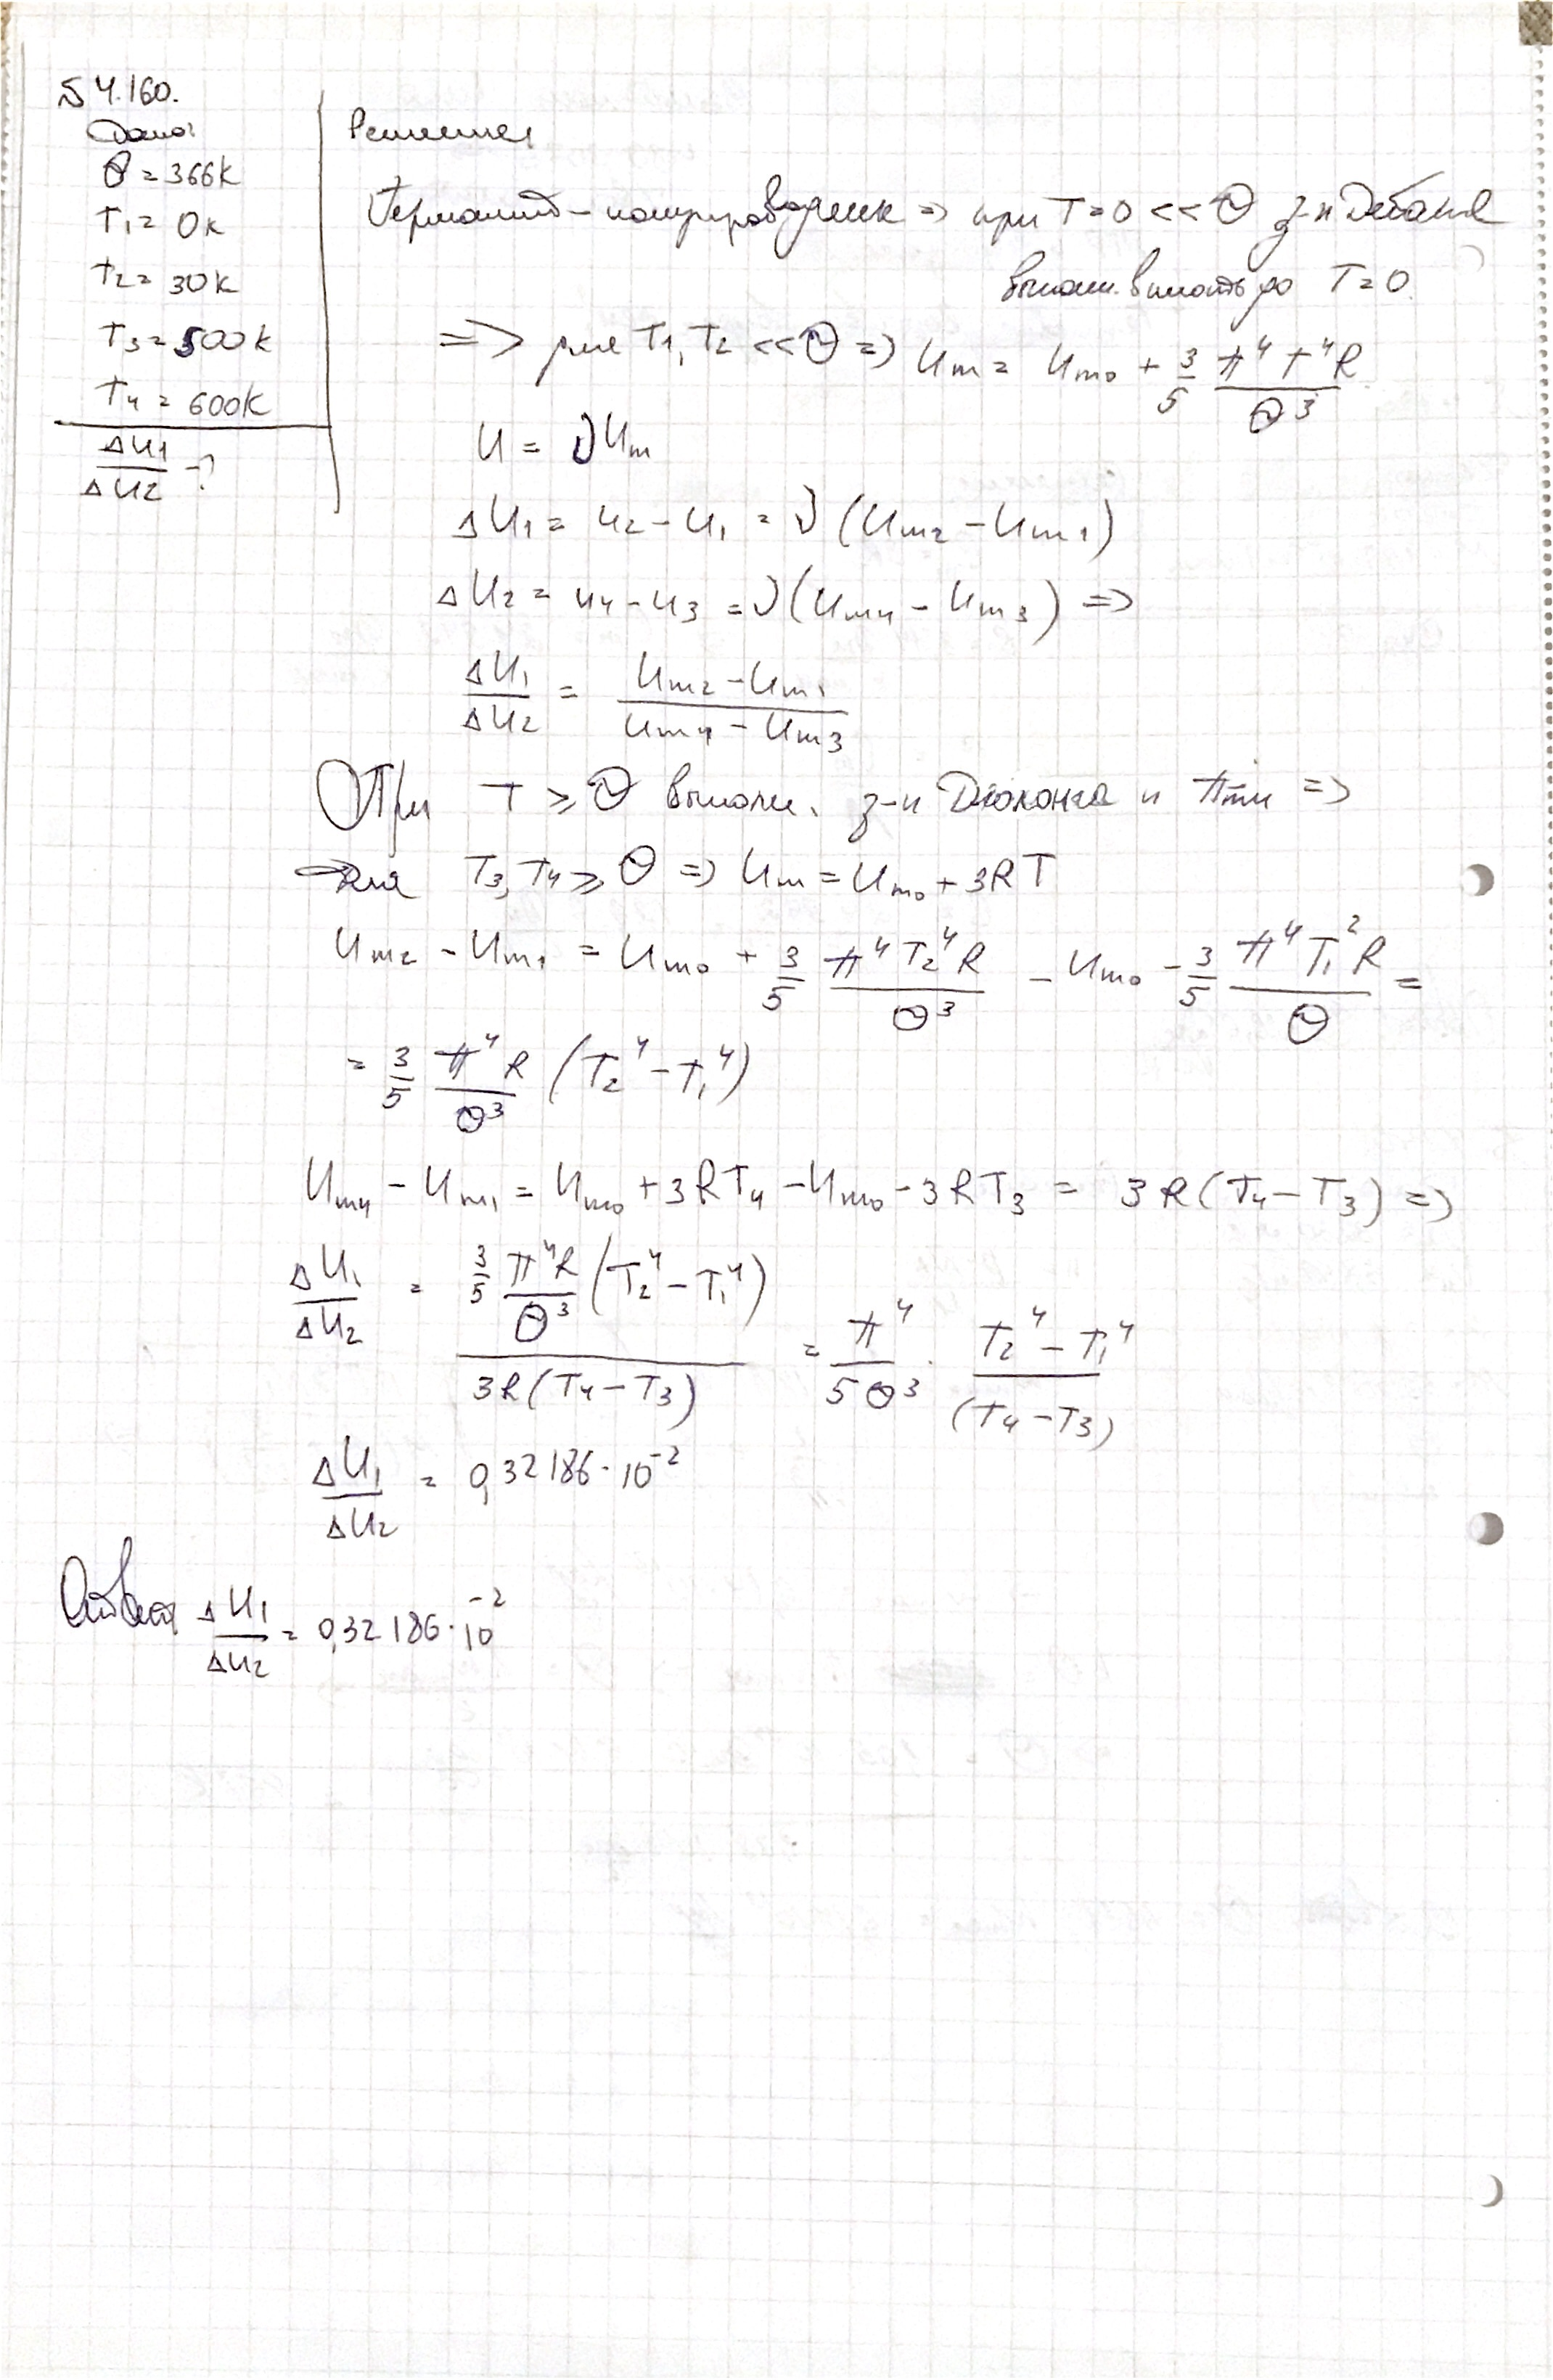
\includegraphics[scale=0.2]{7_2.jpeg}\\
\end{center}
\section{8 раздел}
\begin{center}
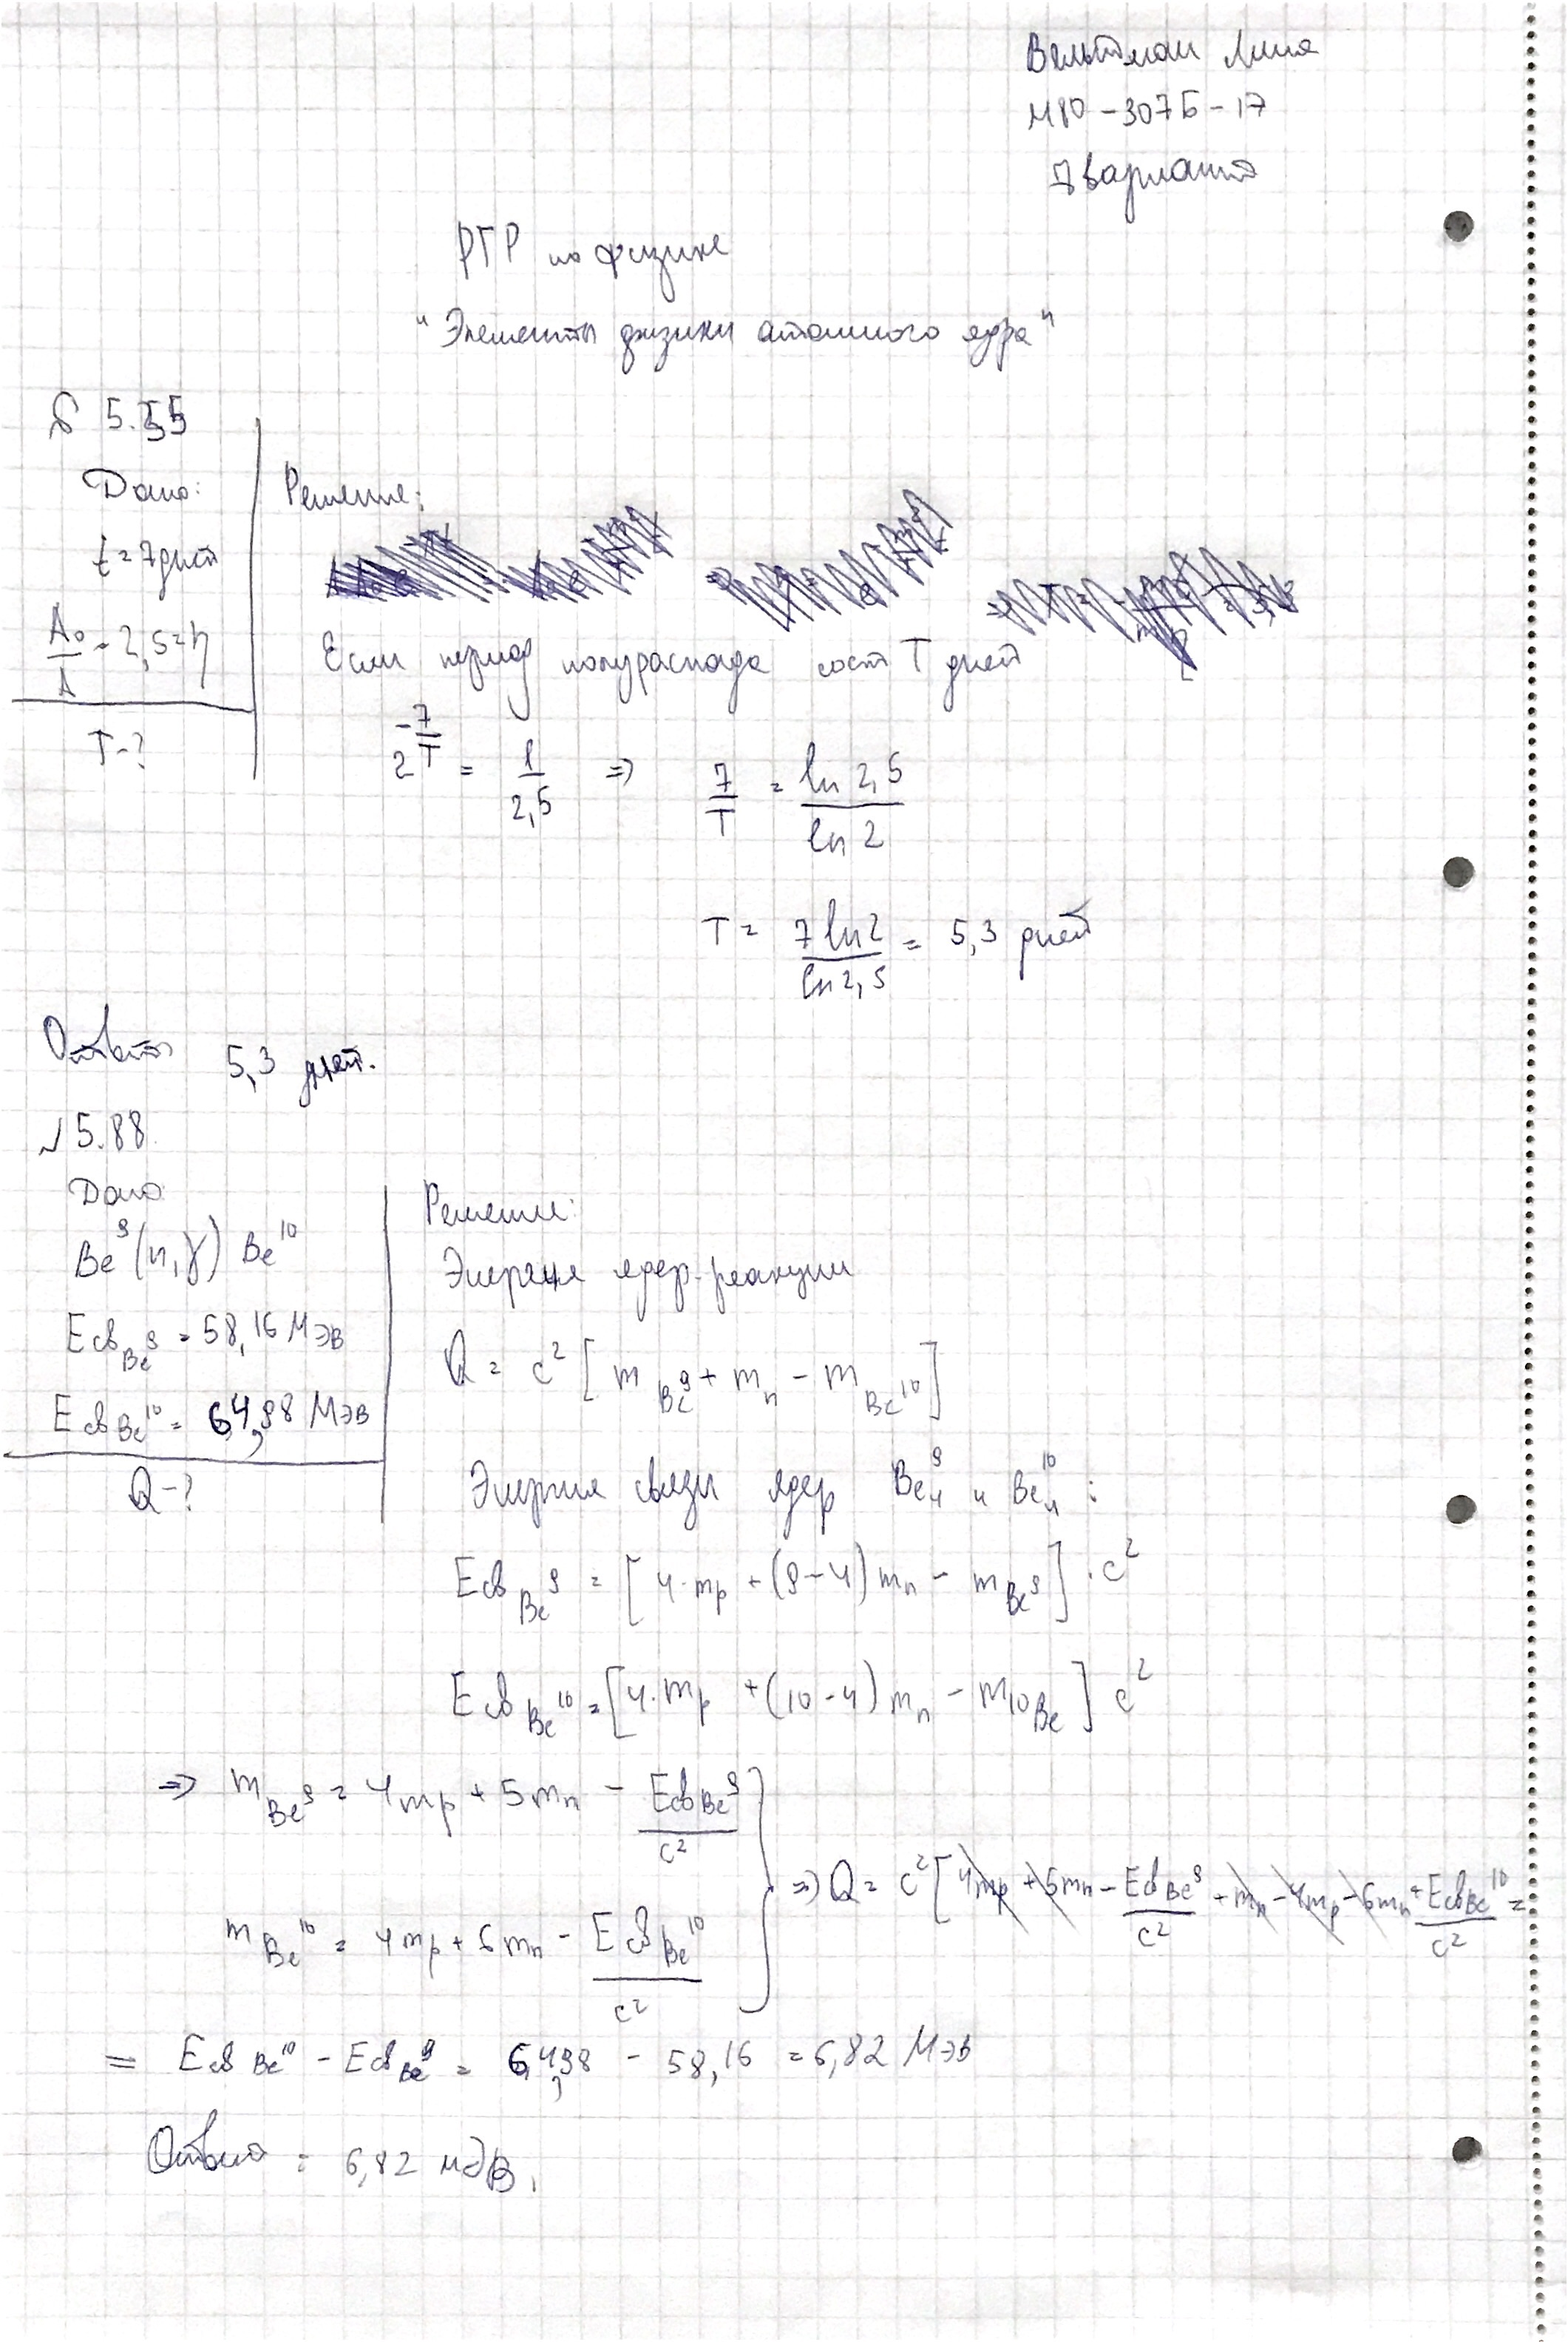
\includegraphics[scale=0.2]{8_1.jpeg}\\
\vfill
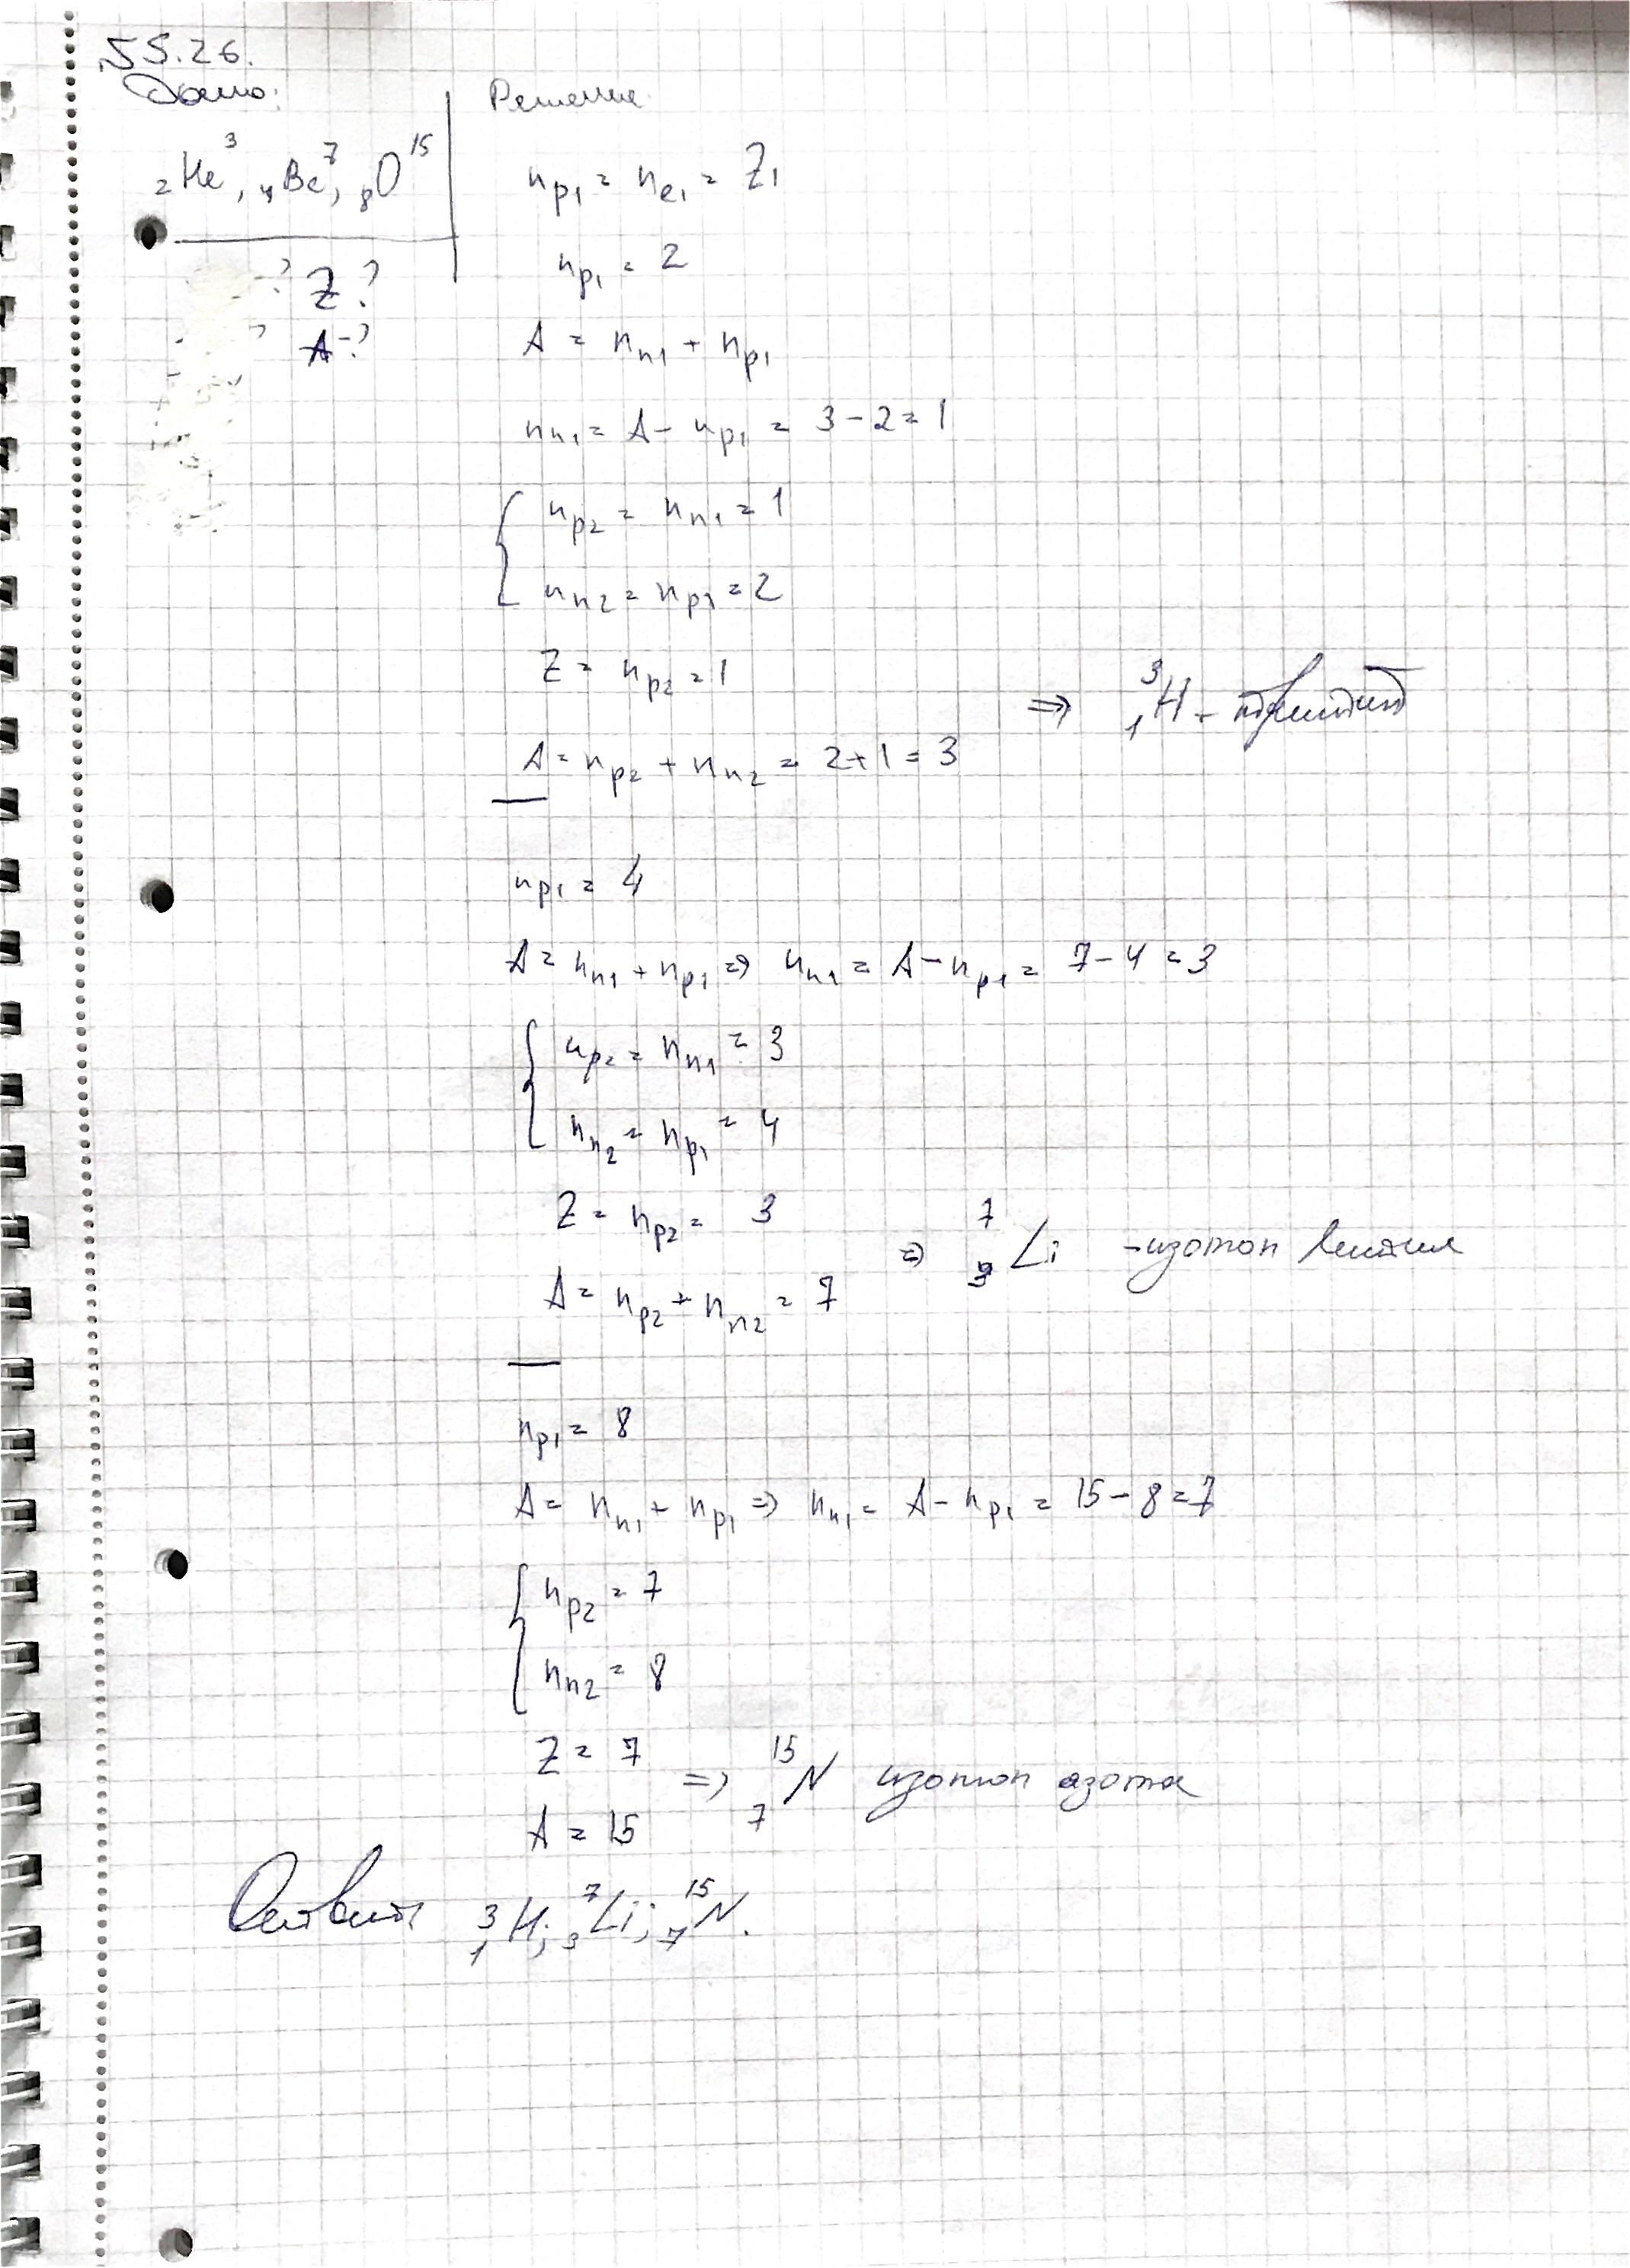
\includegraphics[scale=0.2]{8_2.jpeg}\\
\end{center}


\end{document}